\documentclass{article}
\usepackage{graphicx} % Required for inserting images
\documentclass[11pt]{article}
\usepackage[utf8]{inputenc}
\usepackage{amsmath, amssymb, amsthm}
\usepackage{graphicx}
\usepackage{geometry}
\geometry{margin=1in}
\usepackage{hyperref}
\usepackage{setspace}
\onehalfspacing

\title{The Universal Acceleration Constant: A Unifying Framework for Micro--Macro Energy, Momentum, and Time Dynamics}
\author{Ashleigh Wing \\ Independent Researcher}
\date{21/02/2025}

\begin{document}
\maketitle

\begin{abstract}
I propose a universal framework in which a constant, denoted as \(K^2\), is rigorously derived from the second derivative of an exponential process. This constant serves as a fundamental scaling factor bridging micro-level and macro-level dynamics. By applying a double inversion---transforming exponential functions into their logarithmic counterparts---I demonstrate that energy and momentum transform according to
\[
p_{\text{micro}} = K \cdot p_{\text{macro}} \quad \text{and} \quad E_{\text{micro}} = K^2 \cdot E_{\text{macro}},
\]
thereby replacing heuristic approximations with precise, probabilistic predictions. The framework unifies classical mechanics, general relativity, and quantum mechanics---completing aspects of Einstein's unified field vision and refining black hole thermodynamics via Hawking radiation. Furthermore, by analyzing the acceleration of the inverse (logarithmic) function, the model captures the complete picture of system recycling dynamics, effectively doubling the available correlation information. The universal \(K^2\) framework has transformative applications in astrophysics, fluid dynamics, finance, biology, artificial intelligence, and sustainable energy, and it lays the foundation for a new interdisciplinary field: Unified Systems Dynamics.
\end{abstract}

\section{Introduction}
Bridging the gap between microscopic and macroscopic phenomena has long challenged scientists in physics, economics, biology, and engineering. Traditional models rely on heuristic methods that introduce significant approximations when mapping micro-scale dynamics to macro-scale behavior. In contrast, I propose a novel approach in which a universal constant, \(K^2\), derived from the intrinsic curvature of exponential processes, precisely maps micro-level acceleration to macro-level outcomes. By employing a double inversion that transforms rapid exponential behavior into its slower logarithmic counterpart, my framework not only quantifies the scaling of energy and momentum but also extracts the complete picture of system recycling dynamics. This unified approach refines our theoretical understanding---completing Einstein's vision by replacing force with momentum and energy transformations---and offers transformative practical applications across every field.

\section{Mathematical Derivation from First Principles}
\subsection{Exponential Dynamics and the Emergence of \(K^2\)}
\textbf{Assumption:} At the micro scale, many natural processes are modeled by an exponential function:
\[
f(t) = \exp(-k \cdot t), \quad t \geq 0, \quad k > 0.
\]
This representation, rooted in Euler's formula, is ubiquitous in natural decay and growth phenomena.

\textbf{First Derivative (Rate of Change):}
\[
f'(t) = -k \cdot \exp(-k \cdot t).
\]

\textbf{Second Derivative (Acceleration/Curvature):}
\[
f''(t) = k^2 \cdot \exp(-k \cdot t).
\]
At \(t = 0\), we have:
\[
f(0)=1,\quad f'(0)=-k,\quad f''(0)= k^2.
\]
I define the universal scaling constant as:
\[
K^2 \equiv k^2.
\]
Thus, \(K^2\) represents the instantaneous curvature (acceleration) at \(t = 0\) and forms the foundation of the scaling law.

\subsection{Double Inversion: Bridging Micro and Macro}
Since exponential and logarithmic functions are inverses,
\[
y = \exp(-k \cdot t) \quad \Longrightarrow \quad t = -\frac{1}{k}\ln(y),
\]
this inversion converts rapidly varying micro-scale dynamics into a slowly varying macro-scale logarithmic representation. A subsequent inversion (via a sign change) aligns these scales, establishing that the micro-level acceleration (defined as \(a_{\text{micro}} = f''(t)\)) and the macro-level acceleration (\(a_{\text{macro}}\)) are related by:
\[
a_{\text{micro}} = K^2 \cdot a_{\text{macro}}.
\]
Furthermore, by analyzing the acceleration of the inverse (logarithmic) function, the framework captures the entire recycling dynamics of the system, effectively doubling the available correlation information and providing a complete picture of energy flow. This additional detail is crucial for identifying conditions of maximum flux.

\subsection{Momentum and Energy Scaling}
\textbf{Momentum:} In classical mechanics, momentum is defined as:
\[
p = m \cdot v,
\]
where \(v\) is the velocity (obtained by integrating acceleration). If
\[
a_{\text{micro}} = K^2 \cdot a_{\text{macro}},
\]
and integration over the same time interval yields:
\[
v_{\text{micro}} = K \cdot v_{\text{macro}},
\]
then the micro-level momentum becomes:
\[
p_{\text{micro}} = m \cdot v_{\text{micro}} = K \cdot m \cdot v_{\text{macro}} = K \cdot p_{\text{macro}}.
\]

\textbf{Energy:} Kinetic energy is given by:
\[
E = \frac{1}{2} m v^2.
\]
Substituting \(v_{\text{micro}} = K \cdot v_{\text{macro}}\), we obtain:
\[
E_{\text{micro}} = \frac{1}{2} m (K \cdot v_{\text{macro}})^2 = K^2 \cdot \left(\frac{1}{2} m v_{\text{macro}}^2\right) = K^2 \cdot E_{\text{macro}}.
\]
Thus, the scaling laws are:
\[
p_{\text{micro}} = K \cdot p_{\text{macro}} \quad \text{and} \quad E_{\text{micro}} = K^2 \cdot E_{\text{macro}},
\]
which rigorously establish that \(K^2\) is the universal scaling factor governing momentum and energy transformations between micro- and macro-scale dynamics.

\section{Integration with Established Theories}
\subsection{Relativistic Consistency}
Einstein's field equations are expressed as:
\[
R_{\mu \nu} - \frac{1}{2} R \, g_{\mu \nu} + \Lambda \, g_{\mu \nu} = \frac{8\pi G}{c^4} T_{\mu \nu},
\]
where the stress-energy tensor \(T_{\mu \nu}\) includes energy and momentum densities. With the scaling relations:
\[
p_{\text{micro}} = K \cdot p_{\text{macro}} \quad \text{and} \quad E_{\text{micro}} = K^2 \cdot E_{\text{macro}},
\]
the micro-level contributions in \(T_{\mu \nu}\) are quantitatively linked to the macroscopic curvature via \(K^2\). This provides a precise bridge between quantum fluctuations and classical gravitational fields, thereby refining and completing Einstein's unified field theory.

\subsection{Black Hole Thermodynamics and Hawking Radiation}
For a Schwarzschild black hole, the surface gravity is given by:
\[
\kappa = \frac{1}{4M},
\]
and the Hawking temperature is:
\[
T_H = \frac{\kappa}{2\pi}.
\]
By identifying \(K^2 \sim \kappa^2\), the scaling of energy and momentum governed by \(K^2\) directly influences the thermodynamic properties of black holes. This yields a novel derivation of Hawking radiation, unifying quantum effects with gravitational dynamics.

\subsection{Quantum Mechanical Consistency}
In quantum mechanics, momentum is quantized as:
\[
p = \hbar \cdot k.
\]
Under the \(K^2\) transformation, if:
\[
p_{\text{micro}} = K \cdot p_{\text{macro}},
\]
then the fundamental quantization conditions and Heisenberg's uncertainty principle,
\[
\Delta x \cdot \Delta p \geq \frac{\hbar}{2},
\]
remain invariant across scales. This confirms that the \(K^2\) framework is consistent with established quantum mechanical principles.

\section{Empirical Verification and Visual Evidence}
\subsection{Financial Markets: Antifractal Behavior}
I have observed antifractal behavior using custom spread charts on TradingView. For example, the metric
\[
\frac{(\text{DXY})^2}{\text{XRPUSD}}
\]
displays antifractal characteristics. Screenshots captured at different correlated times provide visual evidence that the inverse log decay of DXY squared (representing its acceleration) is mirrored in XRPUSD. In this study, I have grouped the evidence as follows:
\usepackage % Add this in the preamble, along with your other packages

% In your document, e.g., in Section 4:

\section{Empirical Verification and Visual Evidence}

\subsection*{1-Second Timeframe Screenshots}
\begin{center}
\begin{minipage}{\textwidth}
\centering
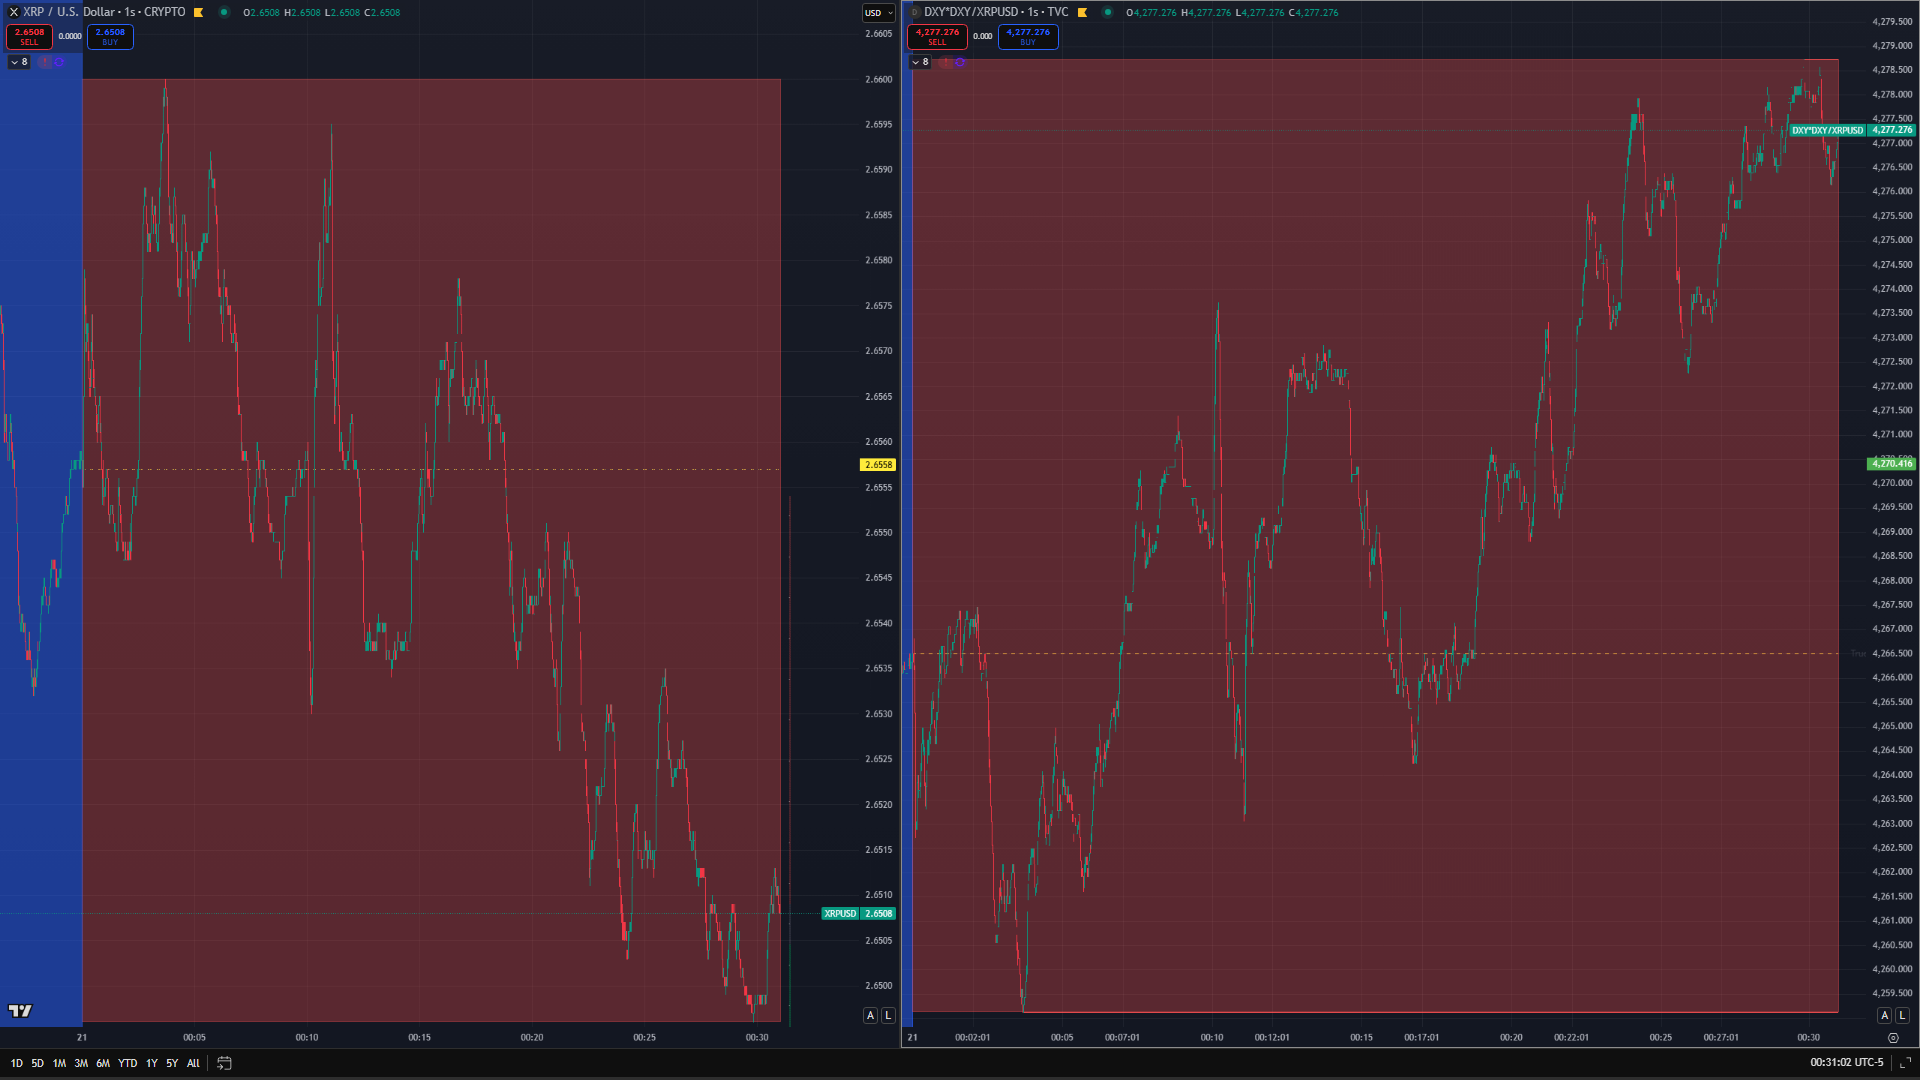
\includegraphics[width=0.3\textwidth]{one_sec_1.png}
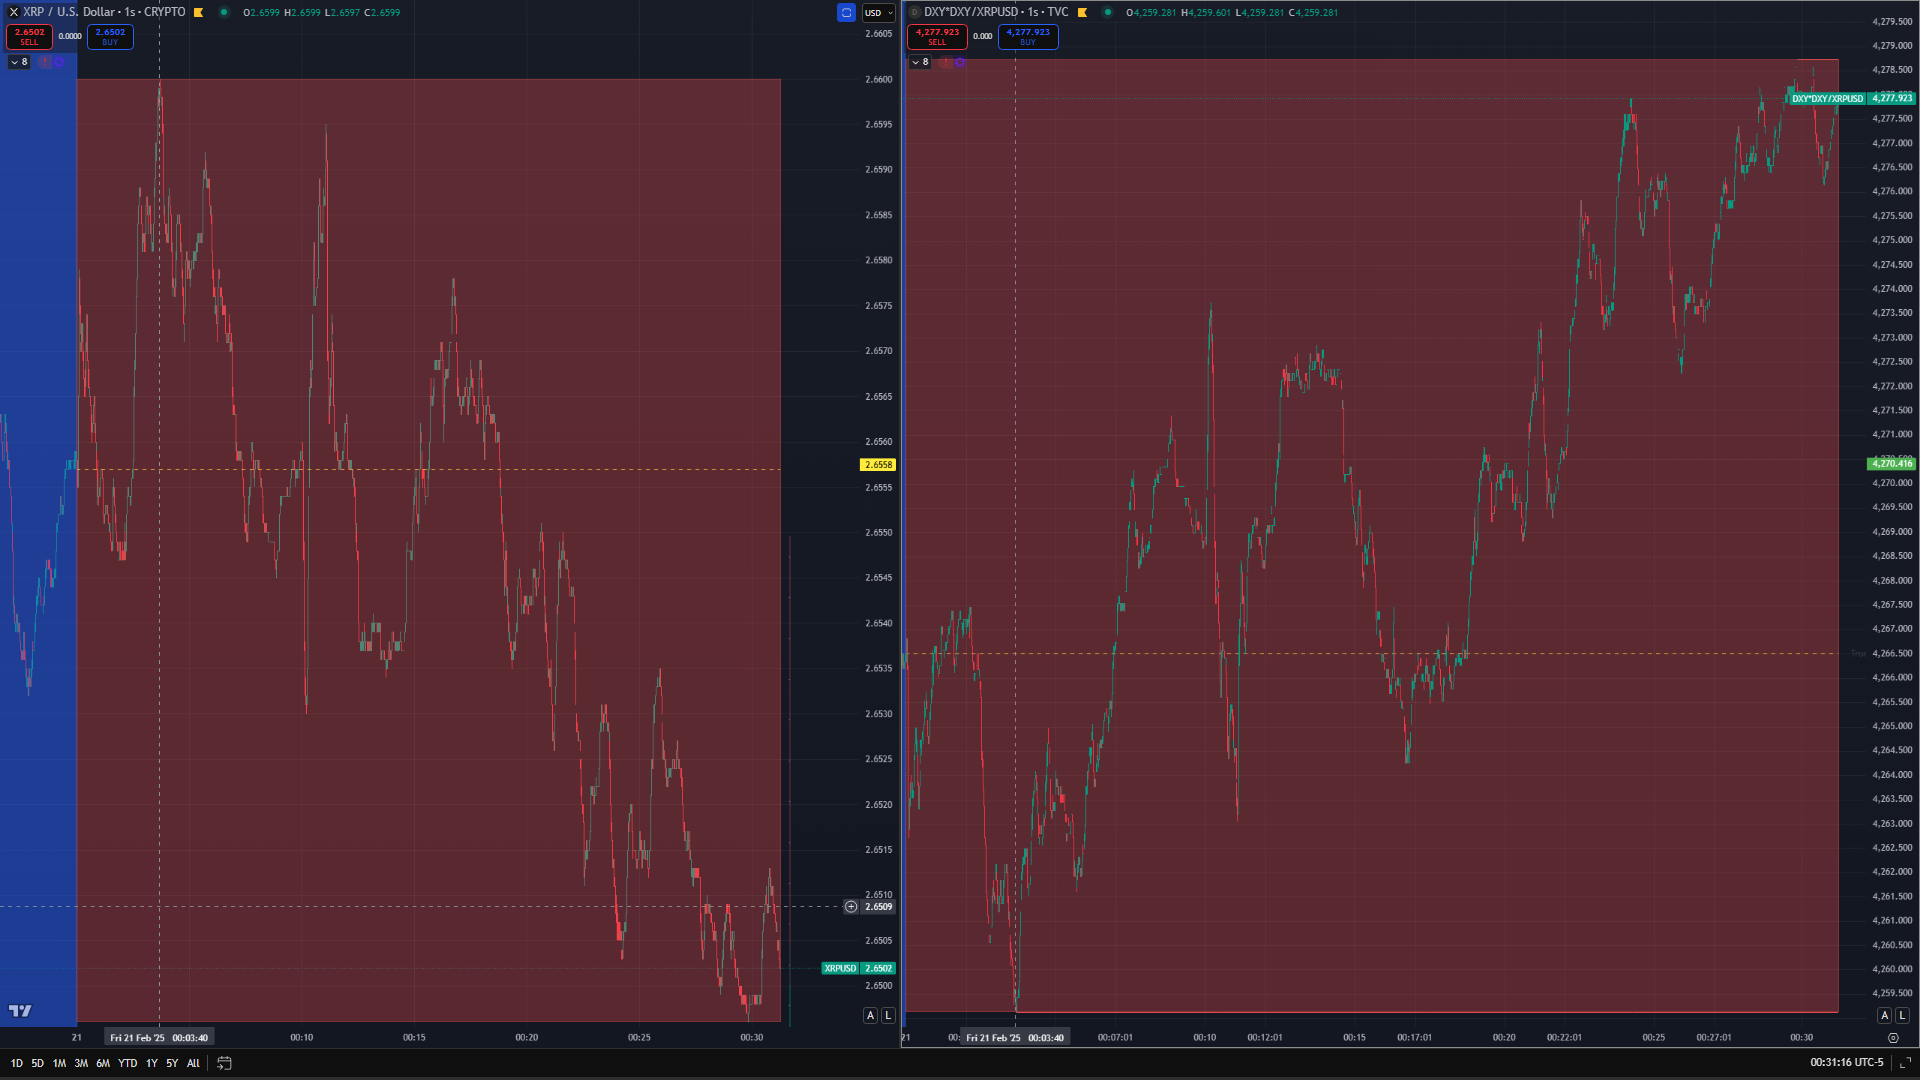
\includegraphics[width=0.3\textwidth]{one_sec_2.png}
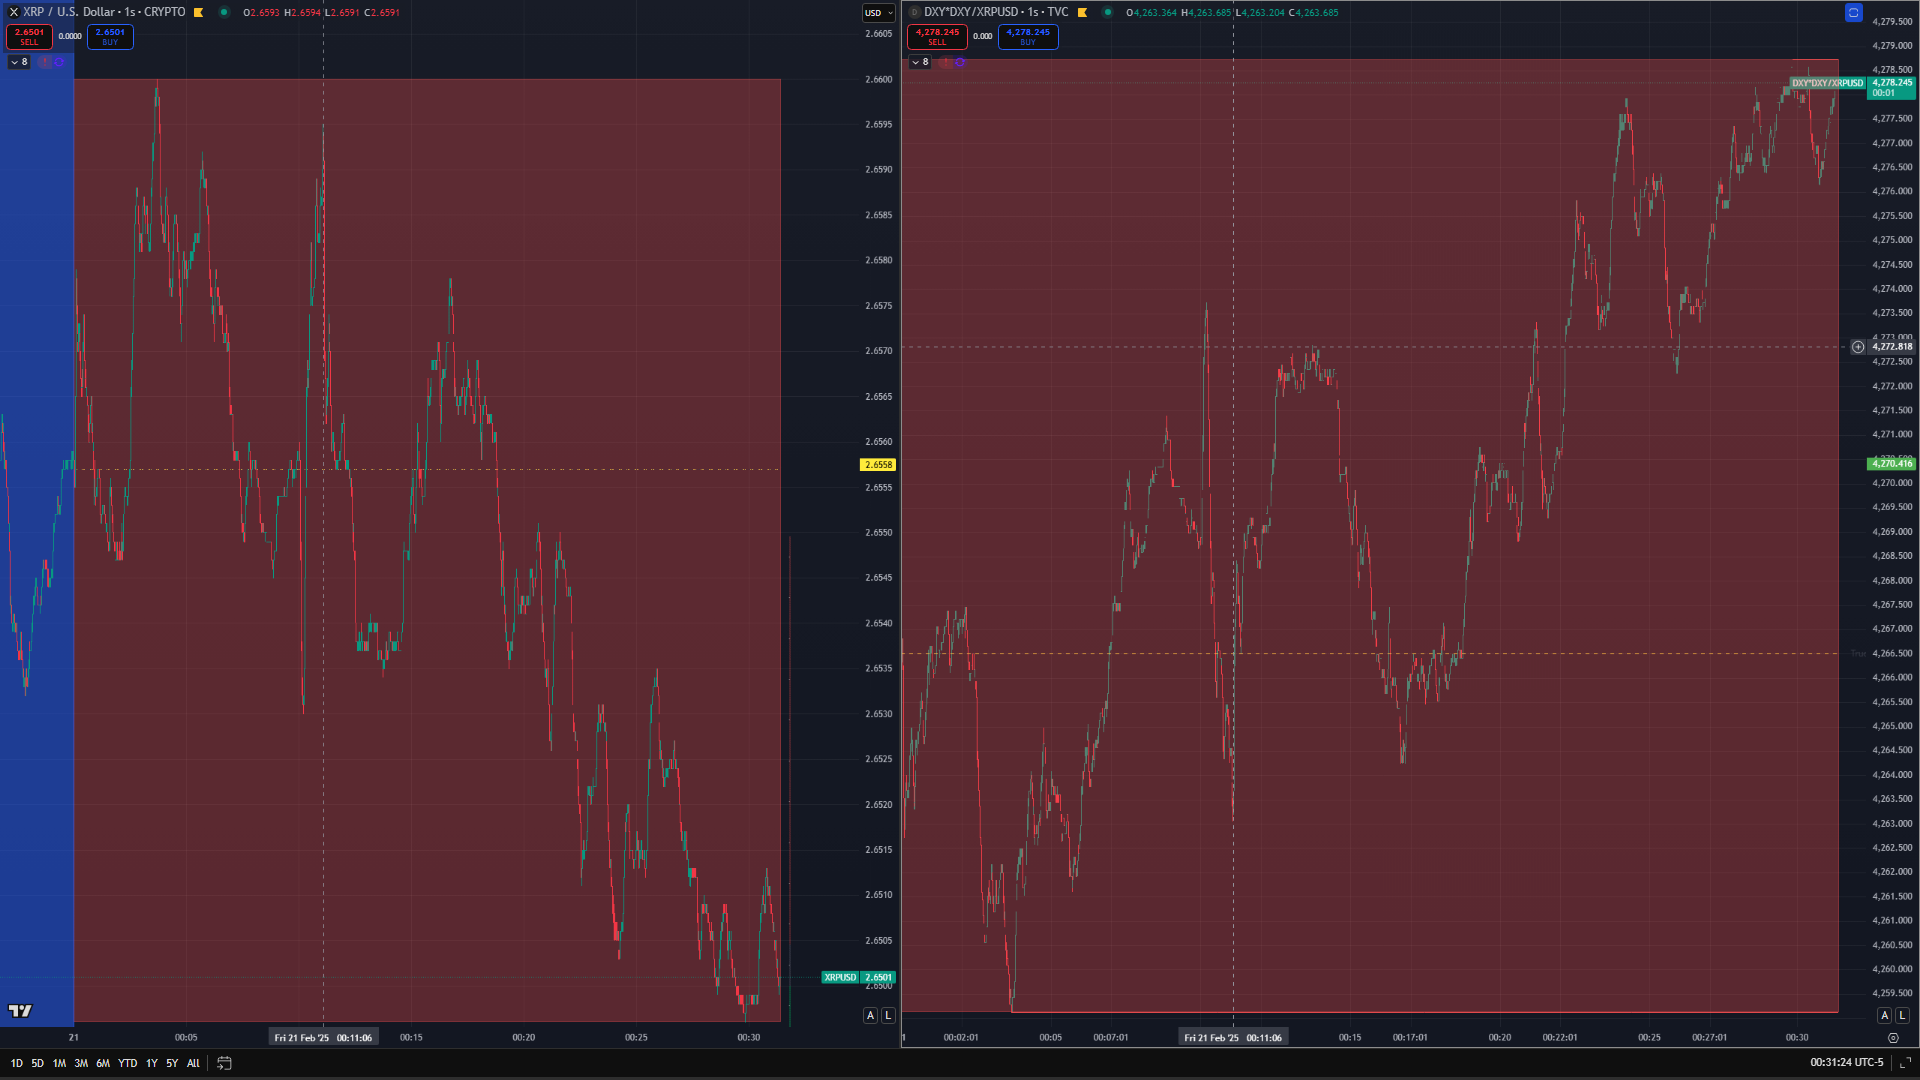
\includegraphics[width=0.3\textwidth]{one_sec_3.png}\\[5mm]
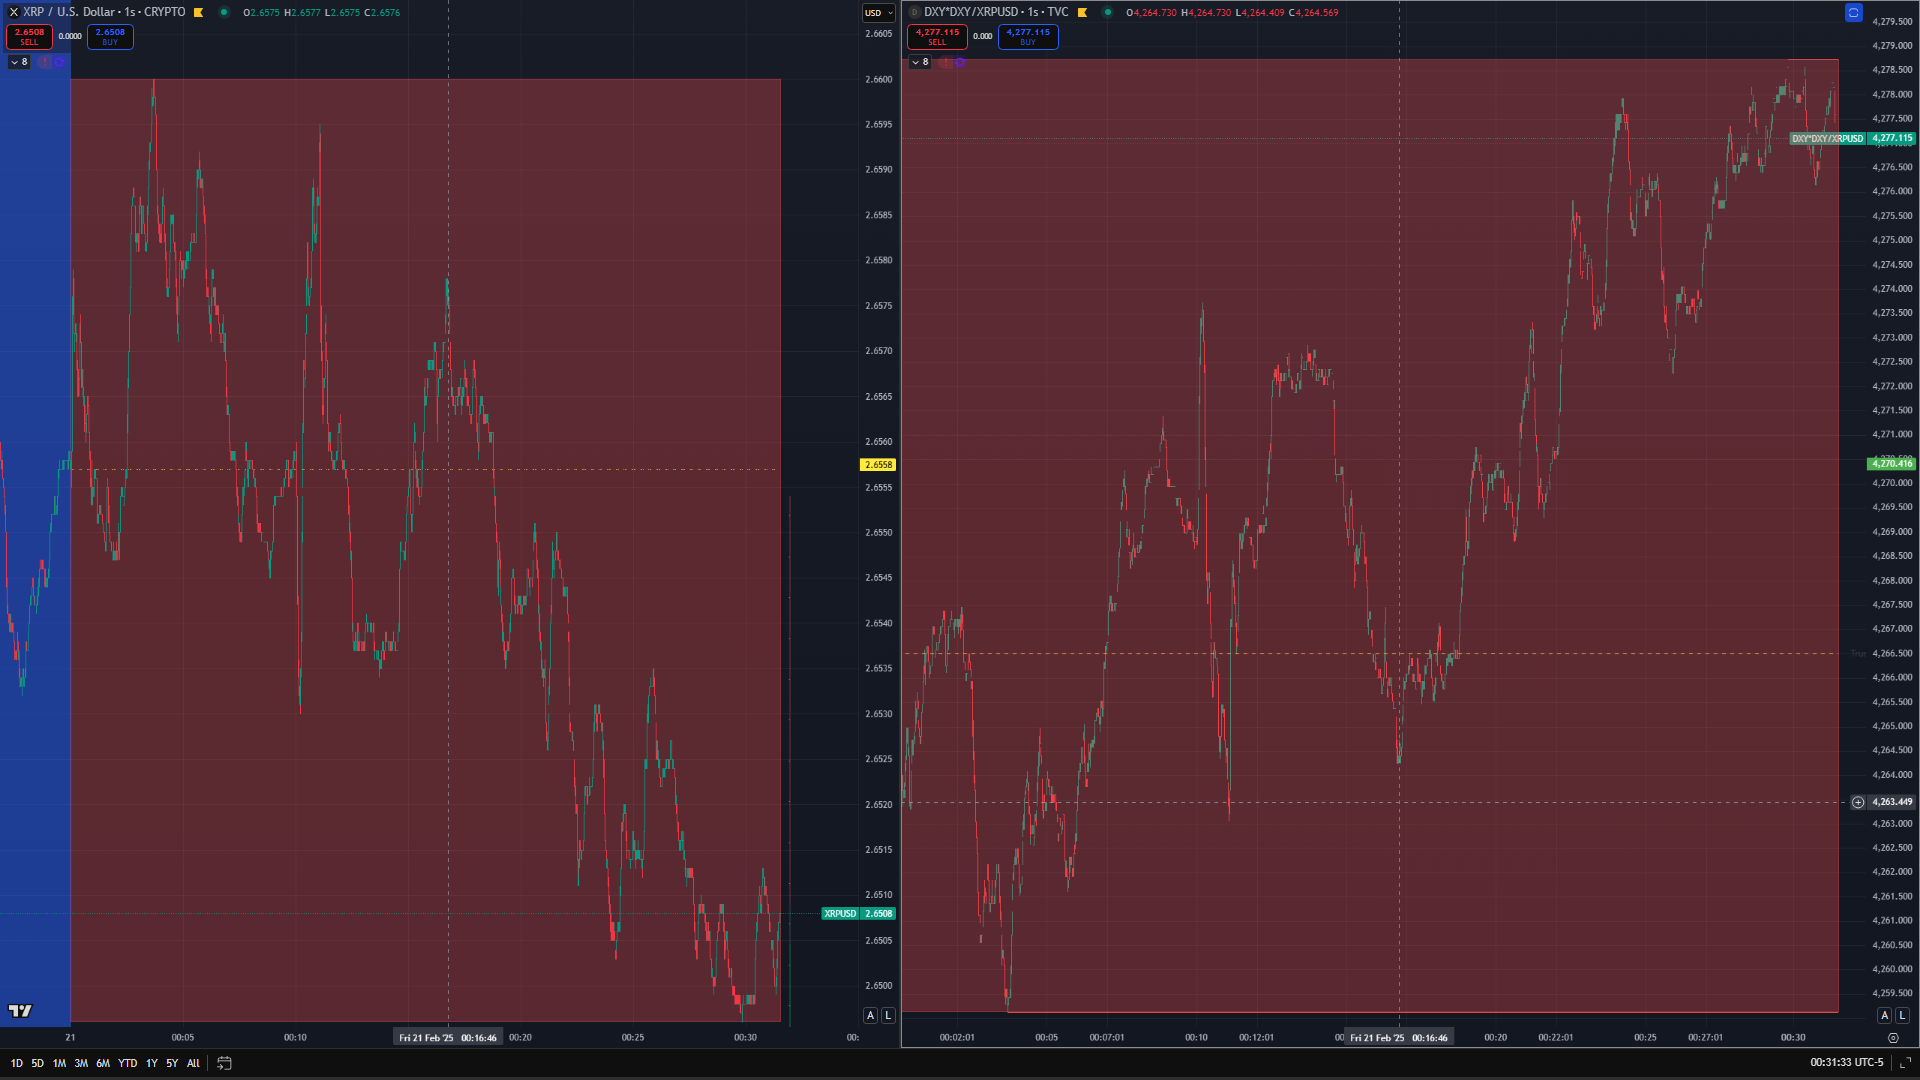
\includegraphics[width=0.3\textwidth]{one_sec_4.png}
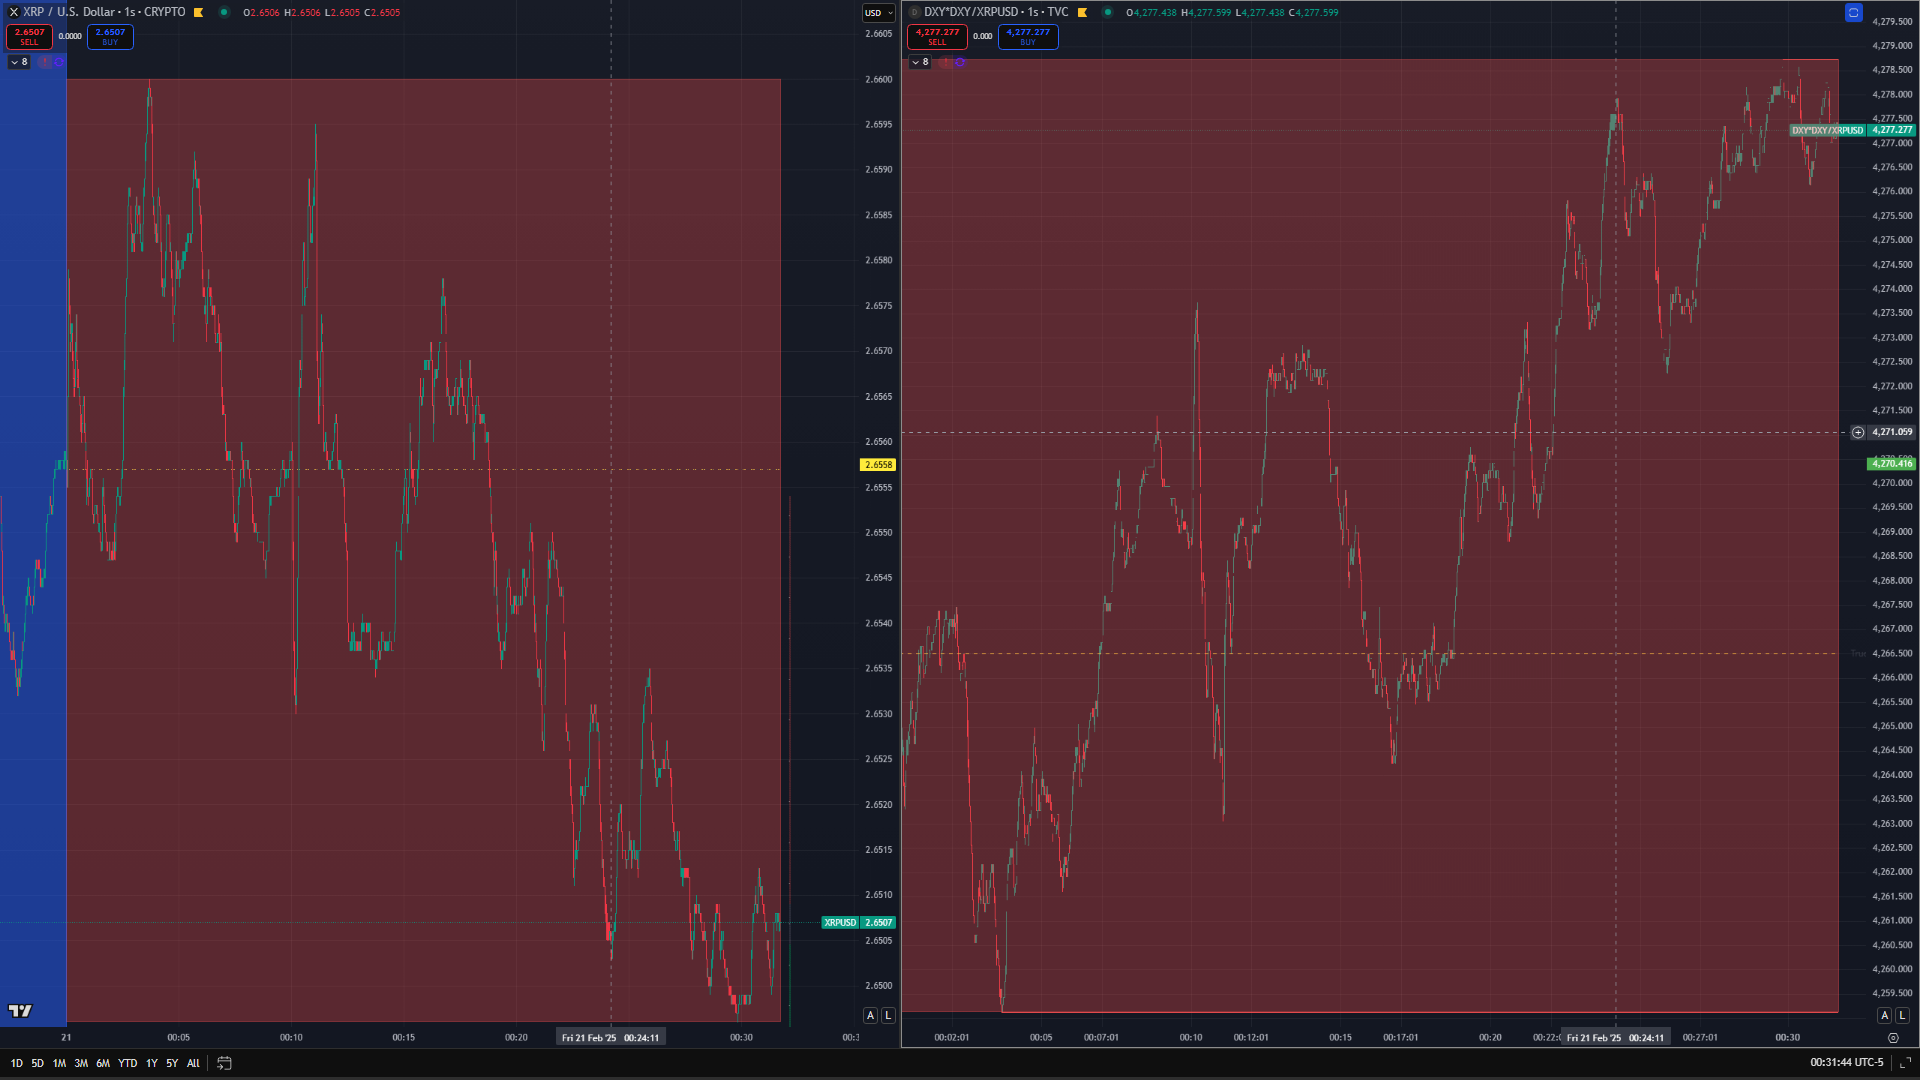
\includegraphics[width=0.3\textwidth]{one_sec_5.png}
\captionof{

Antifractal behavior observed in the (DXY)$^2$/XRPUSD metric at a 1-second timeframe.}
\label{fig:onesec}
\end{minipage}
\end{center}

\subsection*{1-Minute Timeframe Screenshots}
\begin{center}
\begin{minipage}{\textwidth}
\centering
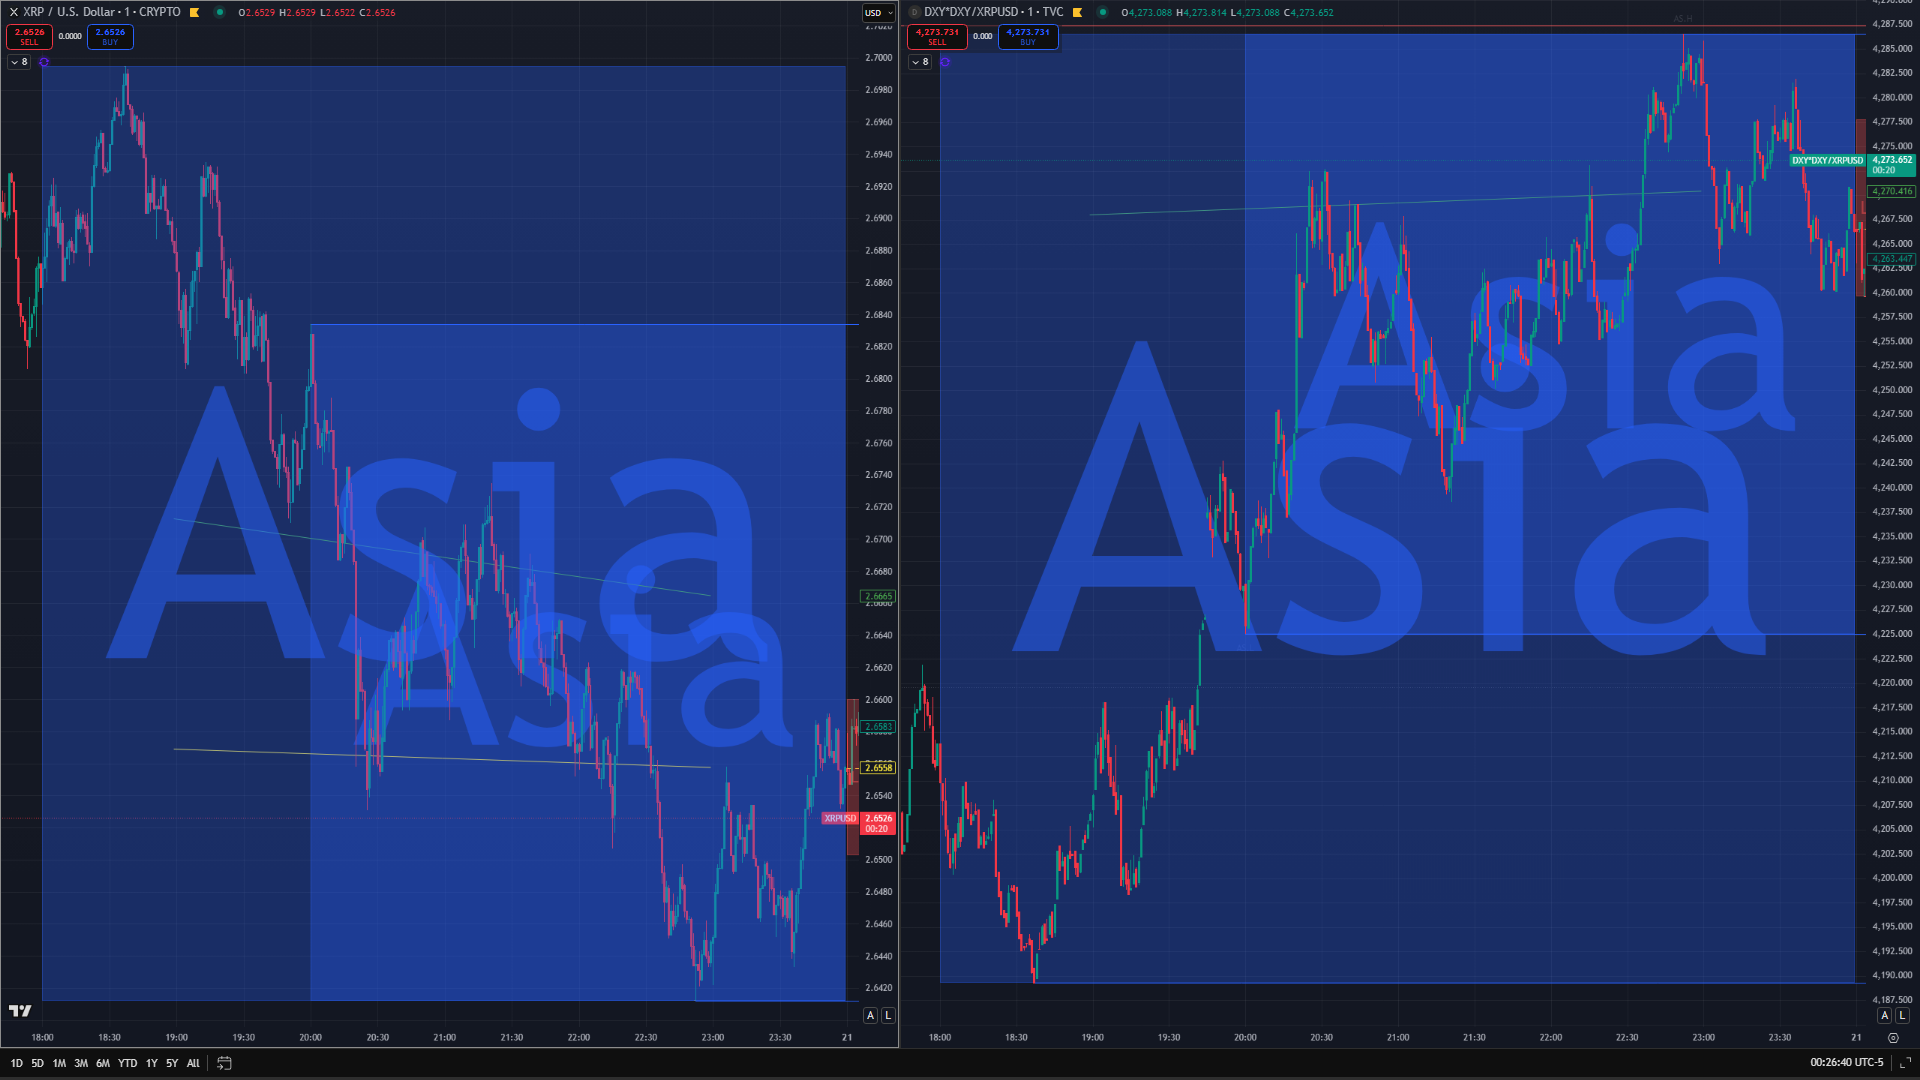
\includegraphics[width=0.3\textwidth]{one_min_1.png}
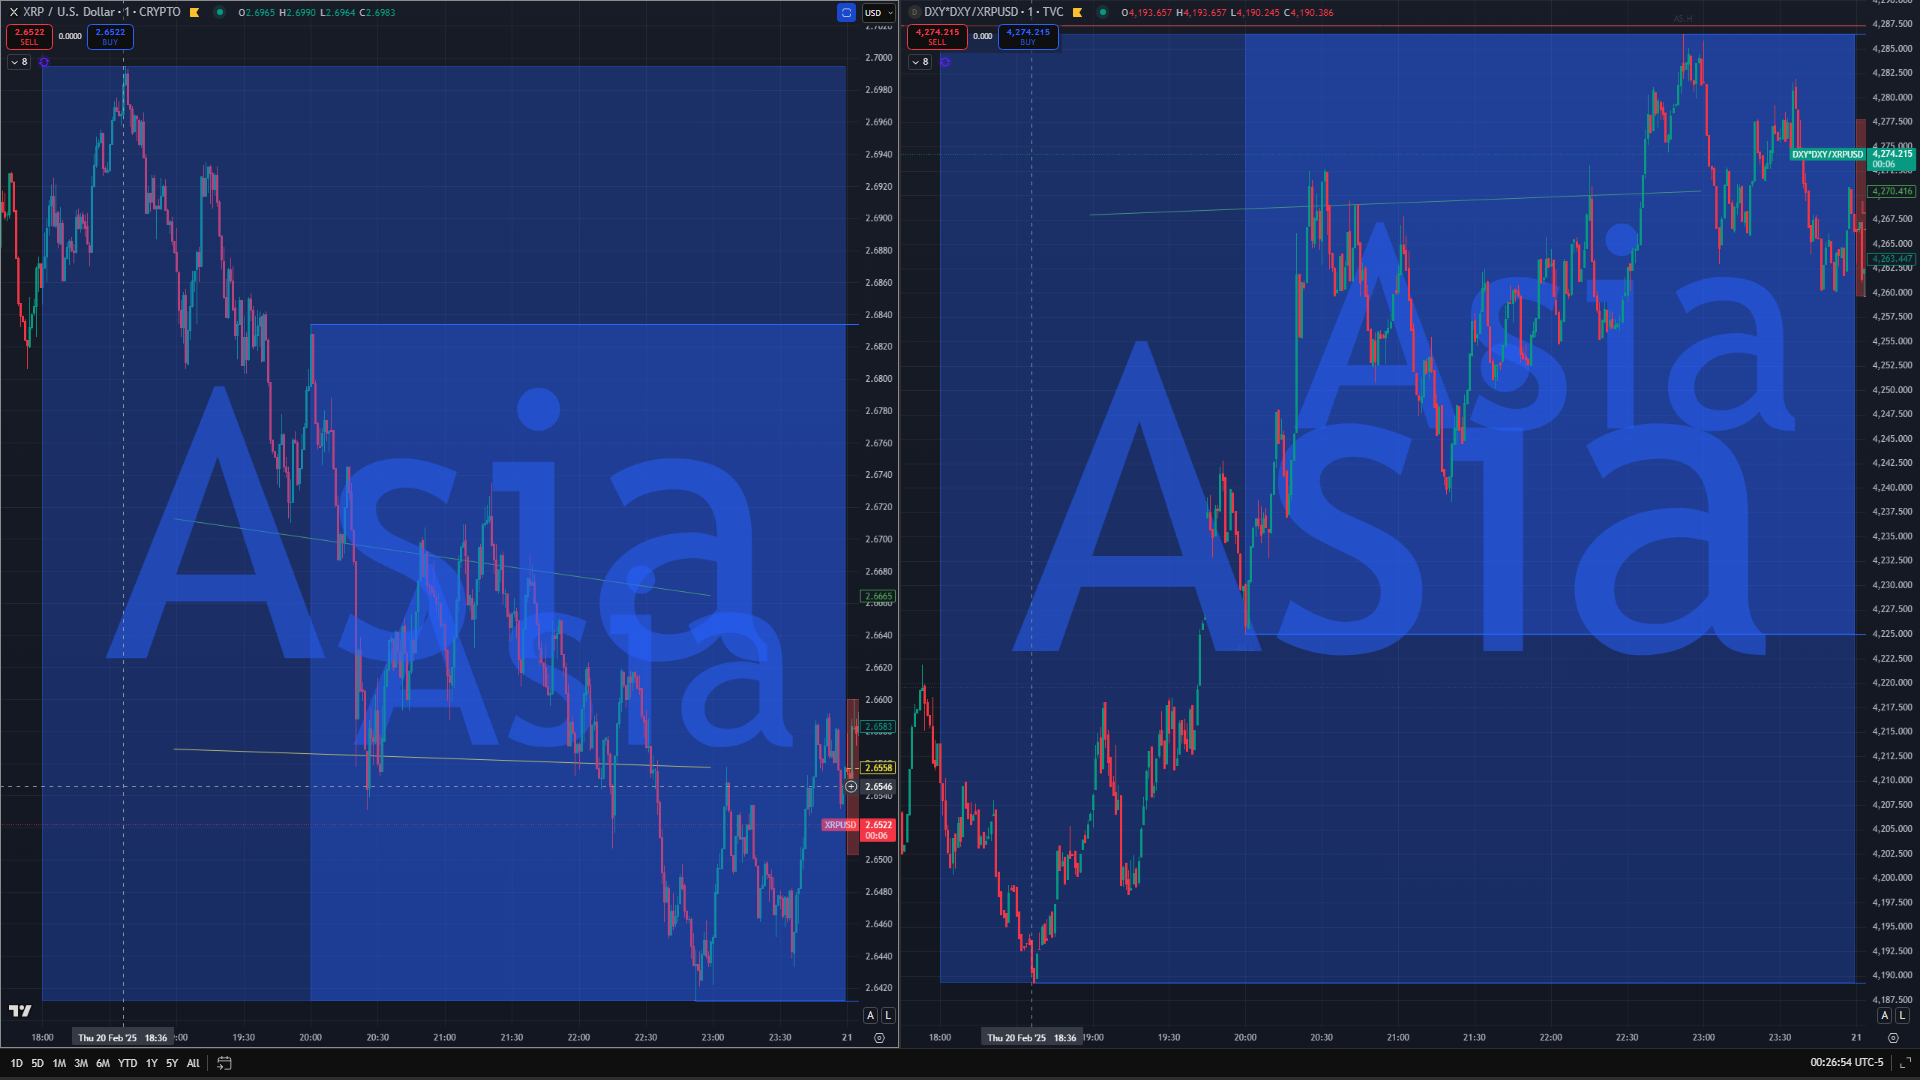
\includegraphics[width=0.3\textwidth]{one_min_2.png}
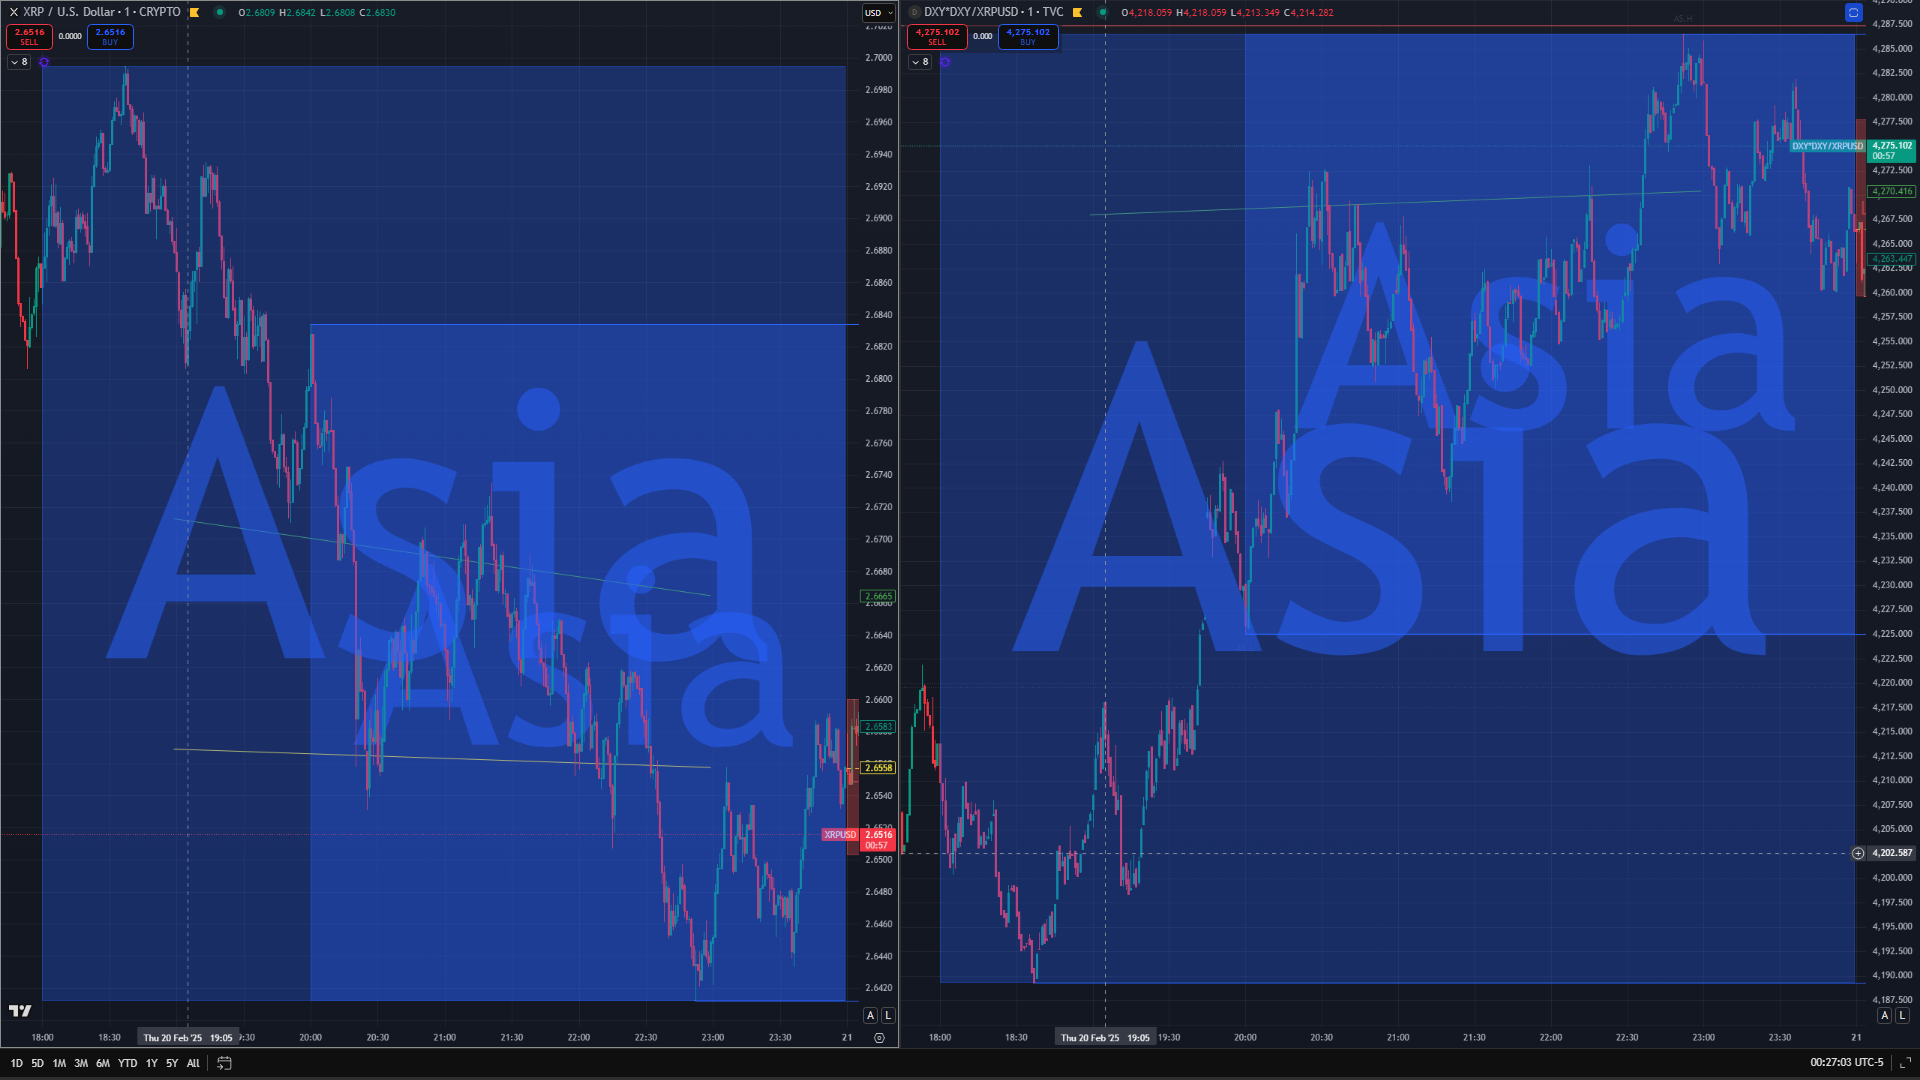
\includegraphics[width=0.3\textwidth]{one_min_3.png}\\[5mm]
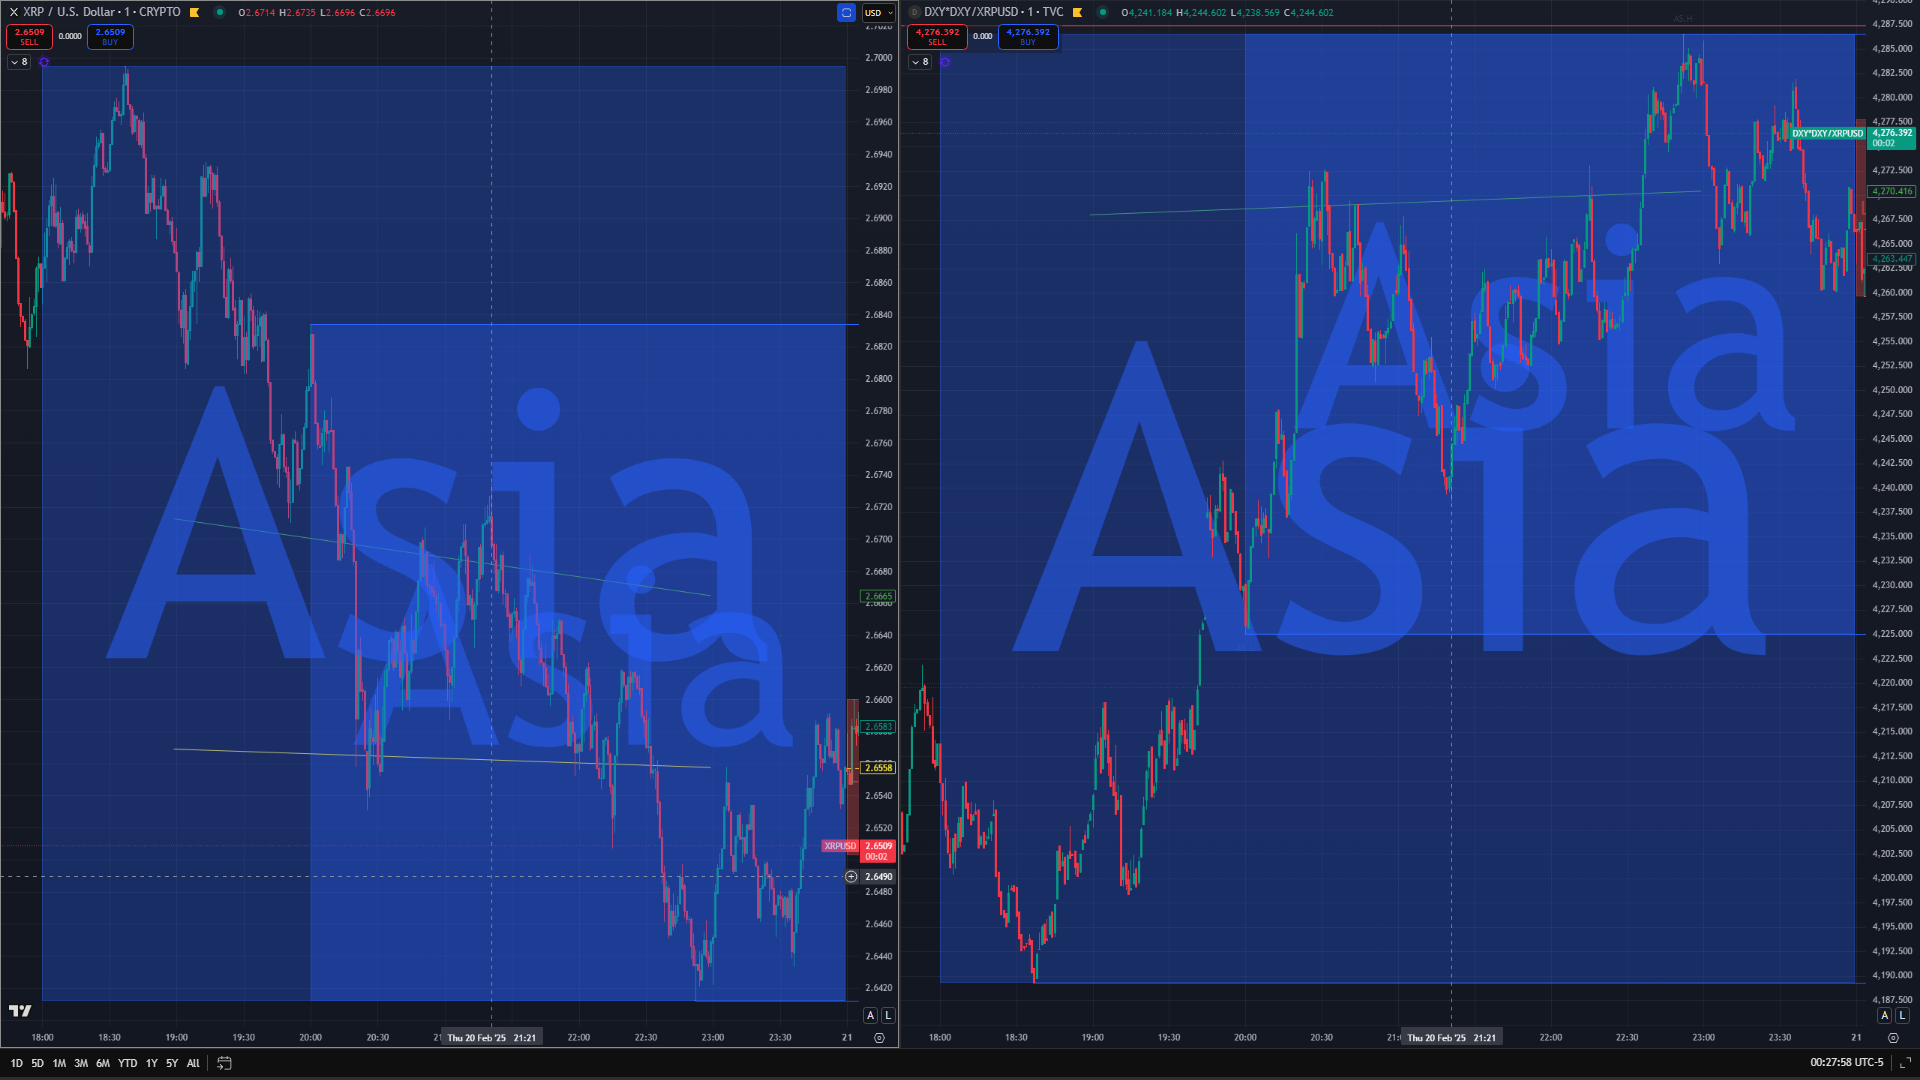
\includegraphics[width=0.3\textwidth]{one_min_4.png}
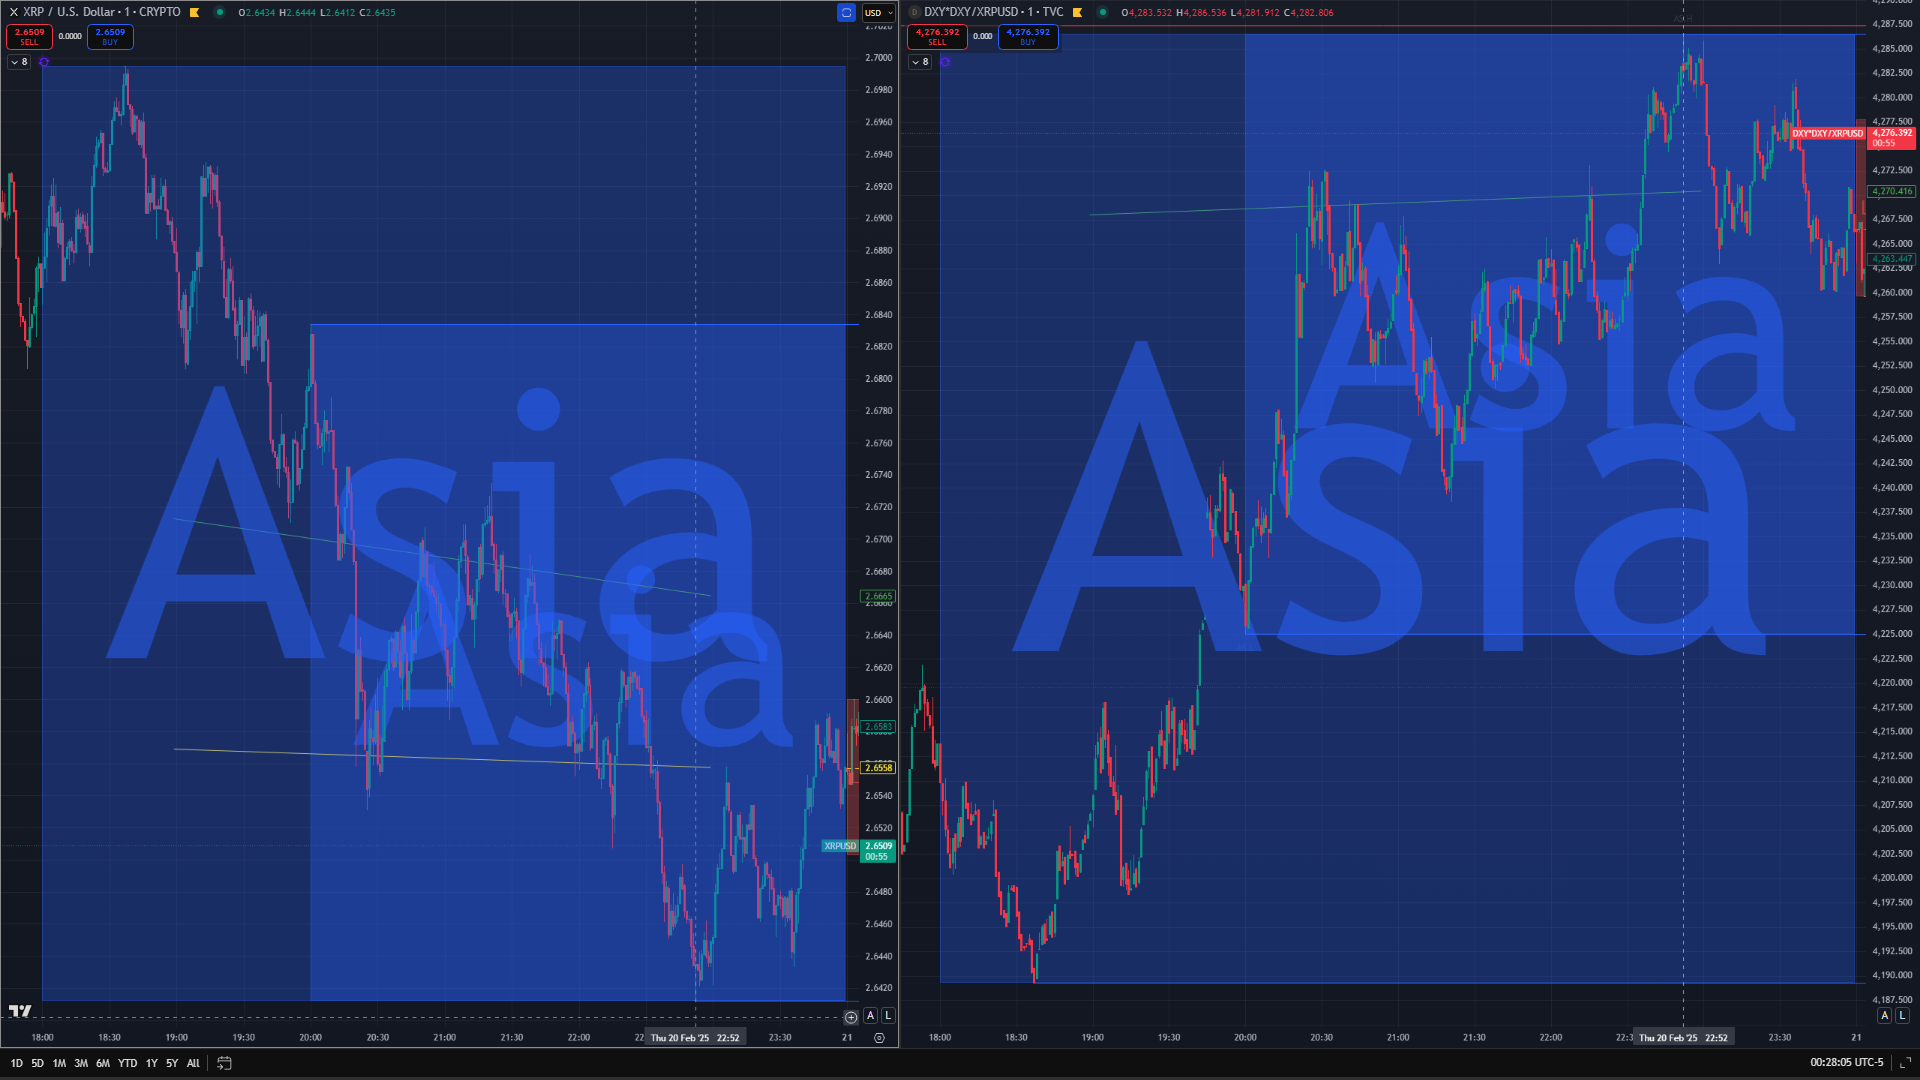
\includegraphics[width=0.3\textwidth]{one_min_5.png}
\captionof{


Antifractal behavior observed in the (DXY)$^2$/XRPUSD metric at a 1-minute timeframe.}
\label{fig:onemin}
\end{minipage}
\end{center}

\subsection*{1-Hour Timeframe Screenshots}
\begin{center}
\begin{minipage}{\textwidth}
\centering
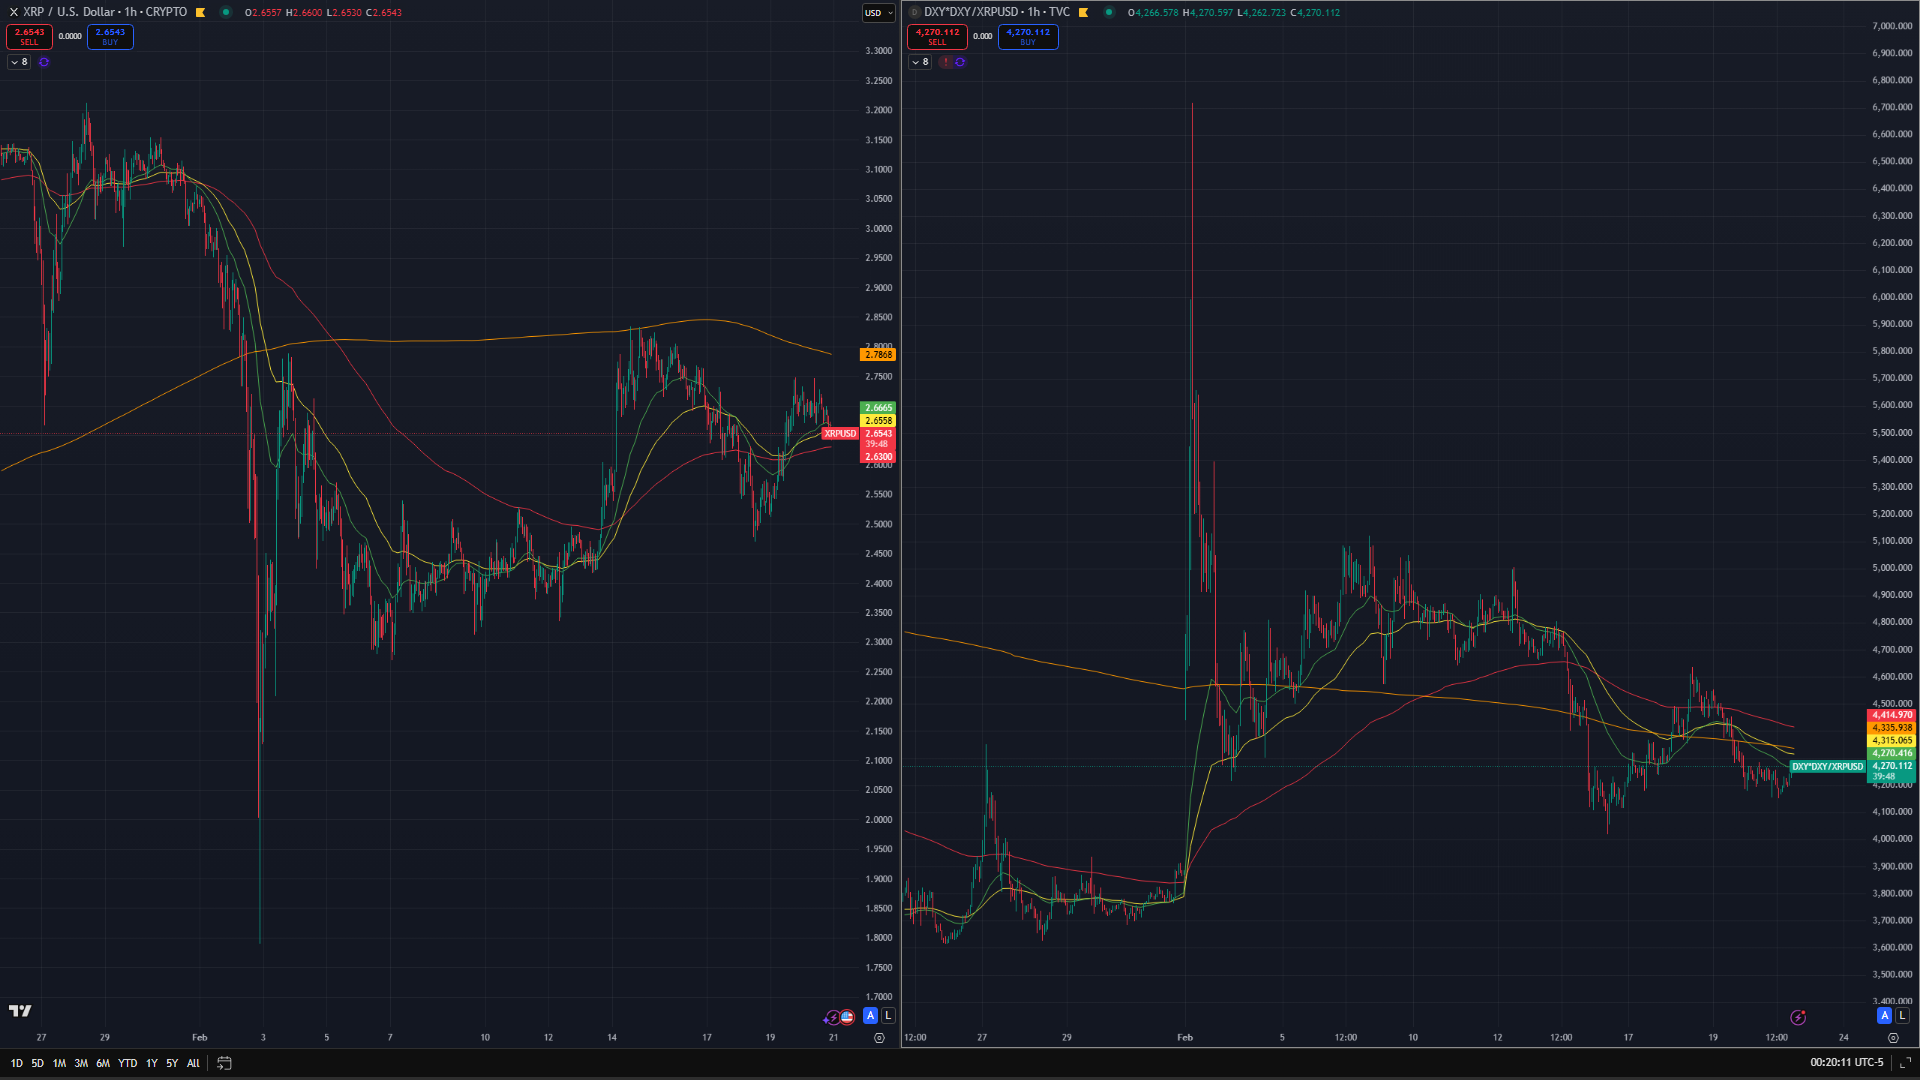
\includegraphics[width=0.3\textwidth]{one_hour_1.png}
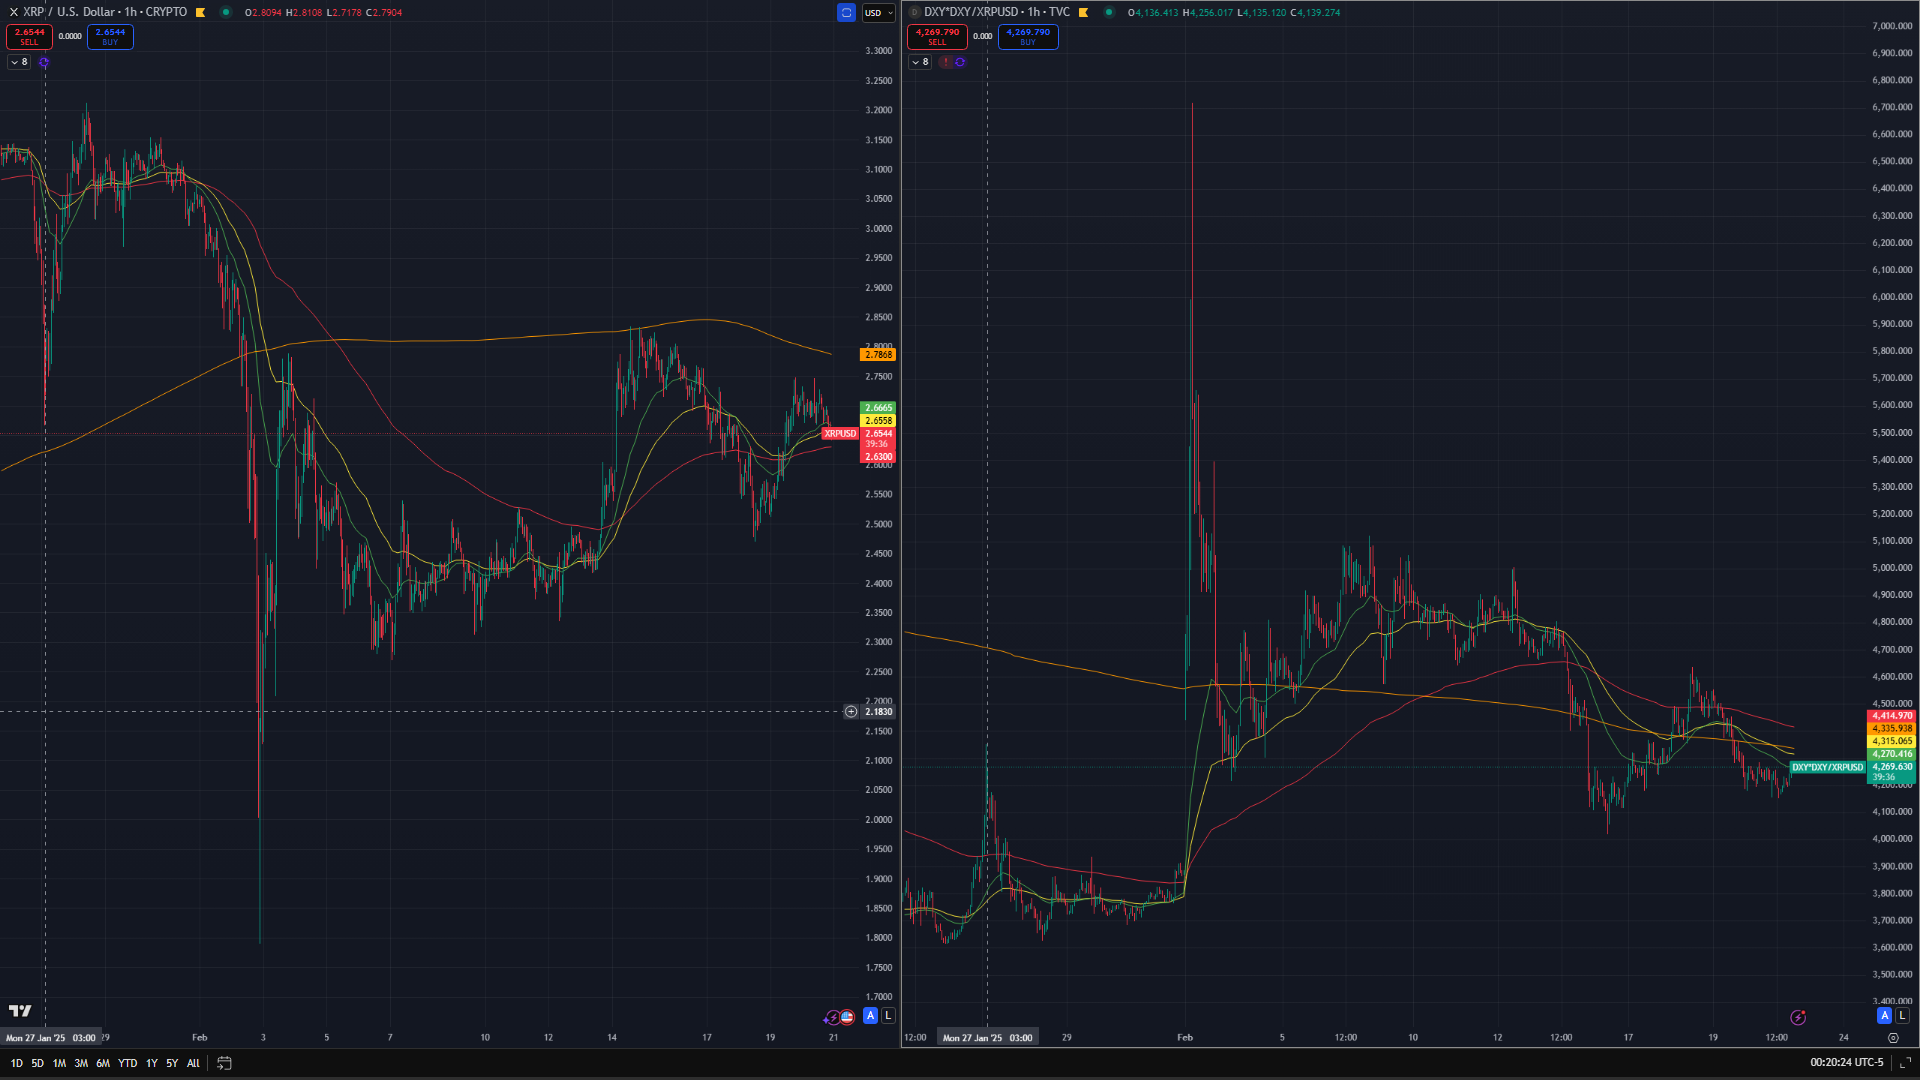
\includegraphics[width=0.3\textwidth]{one_hour_2.png}
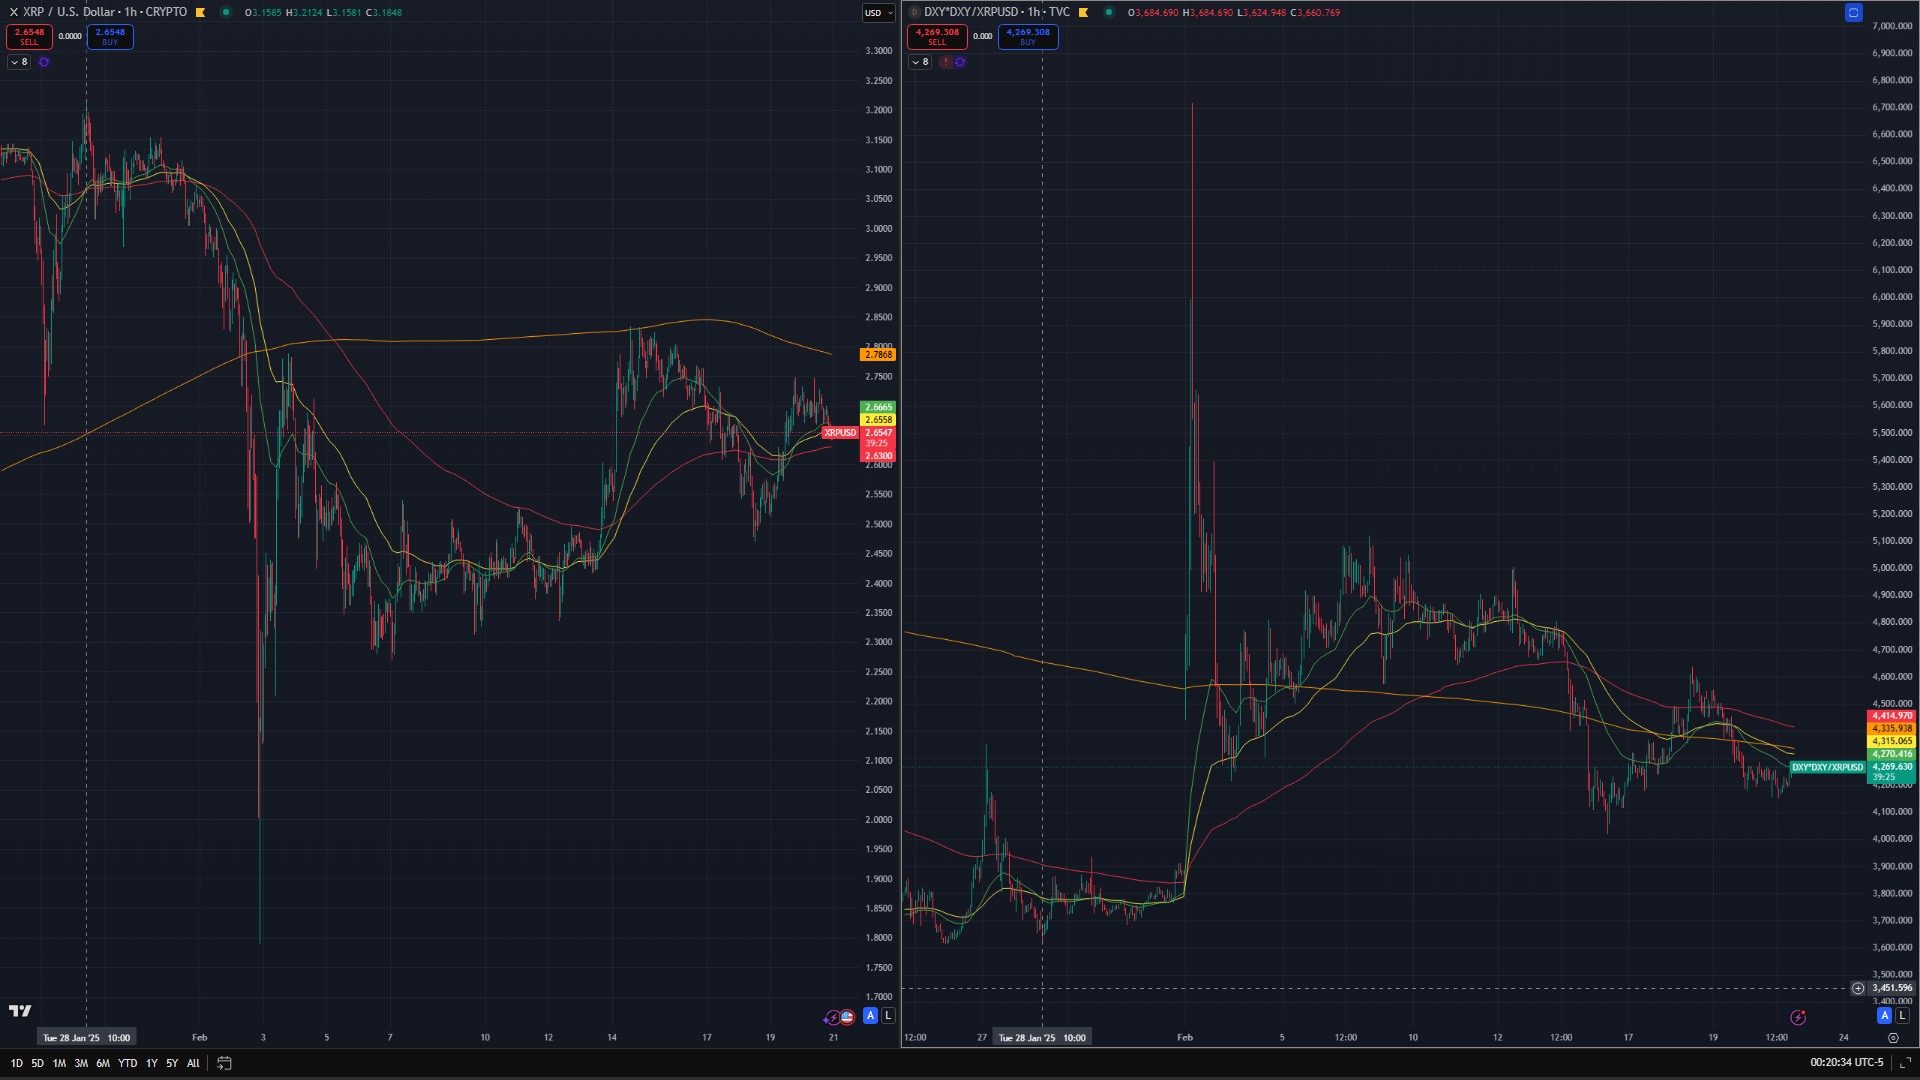
\includegraphics[width=0.3\textwidth]{one_hour_3.png}\\[5mm]
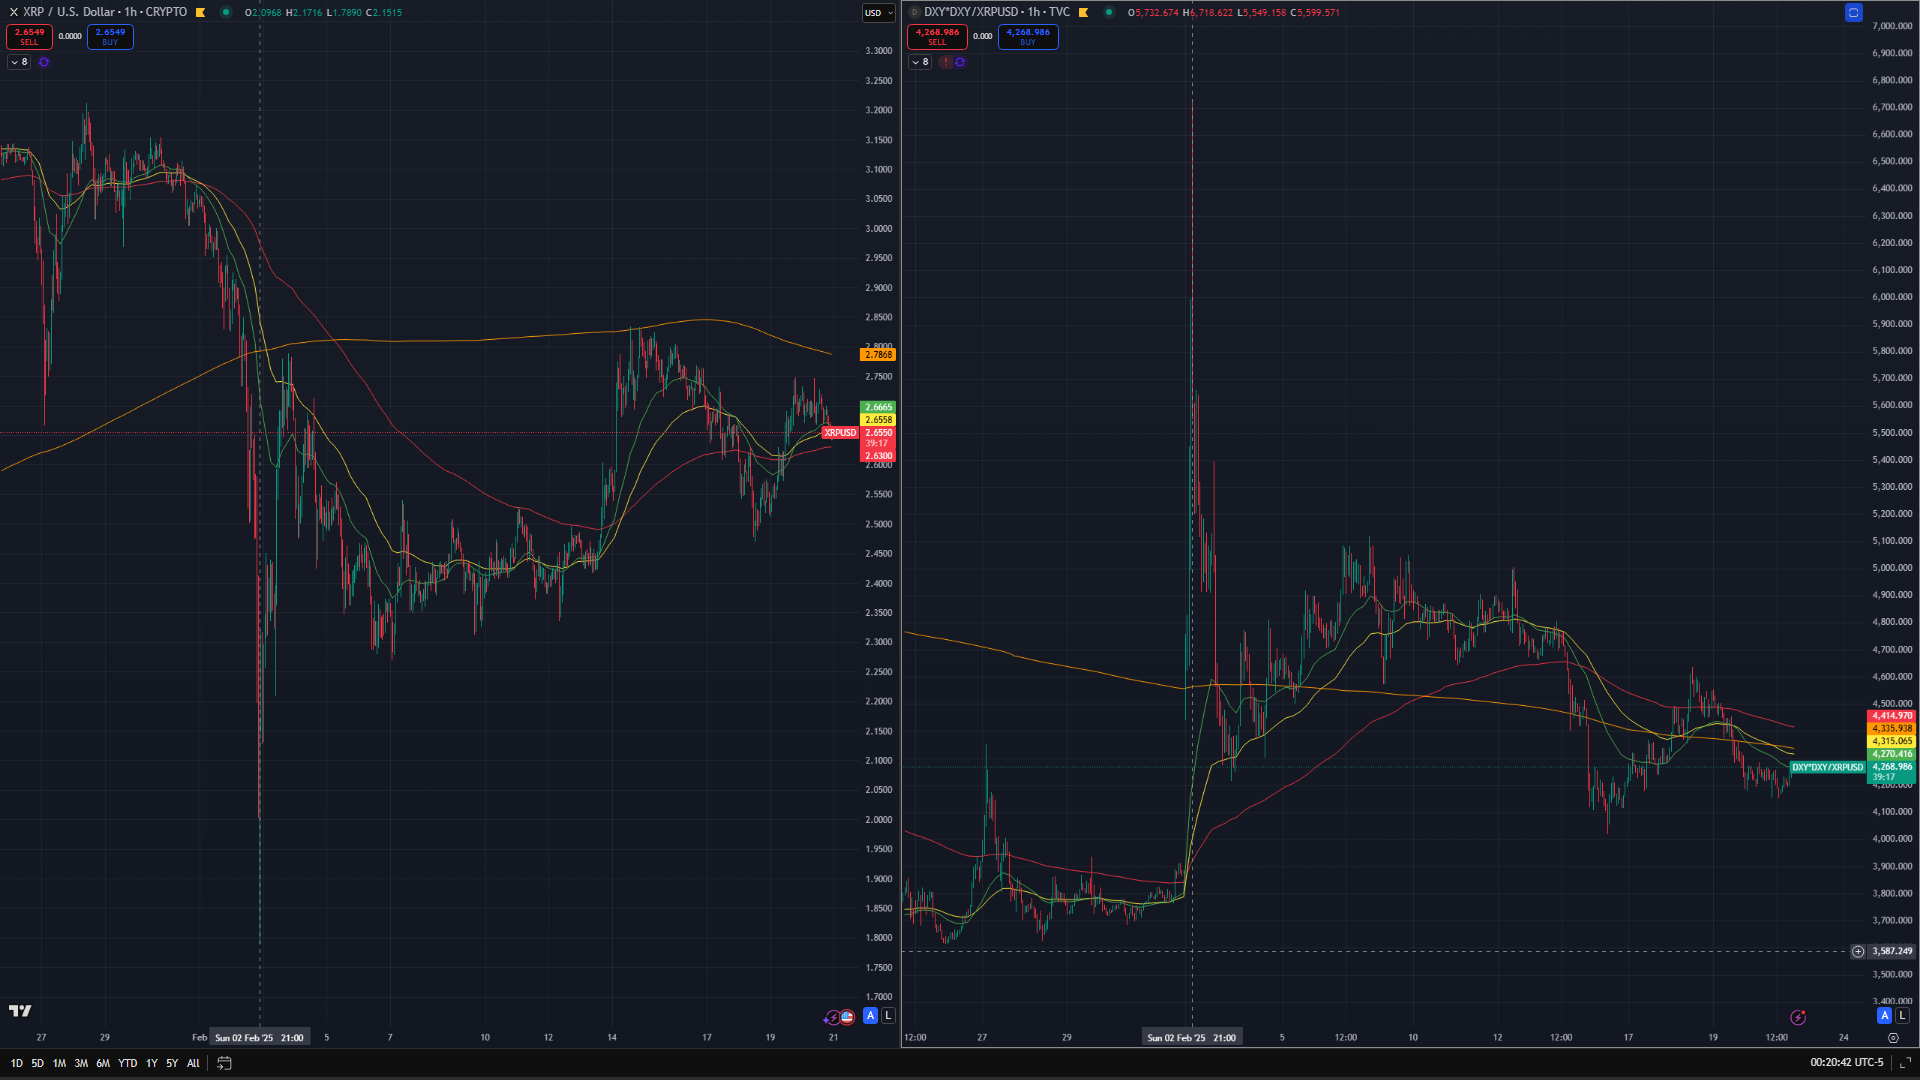
\includegraphics[width=0.3\textwidth]{one_hour_4.png}
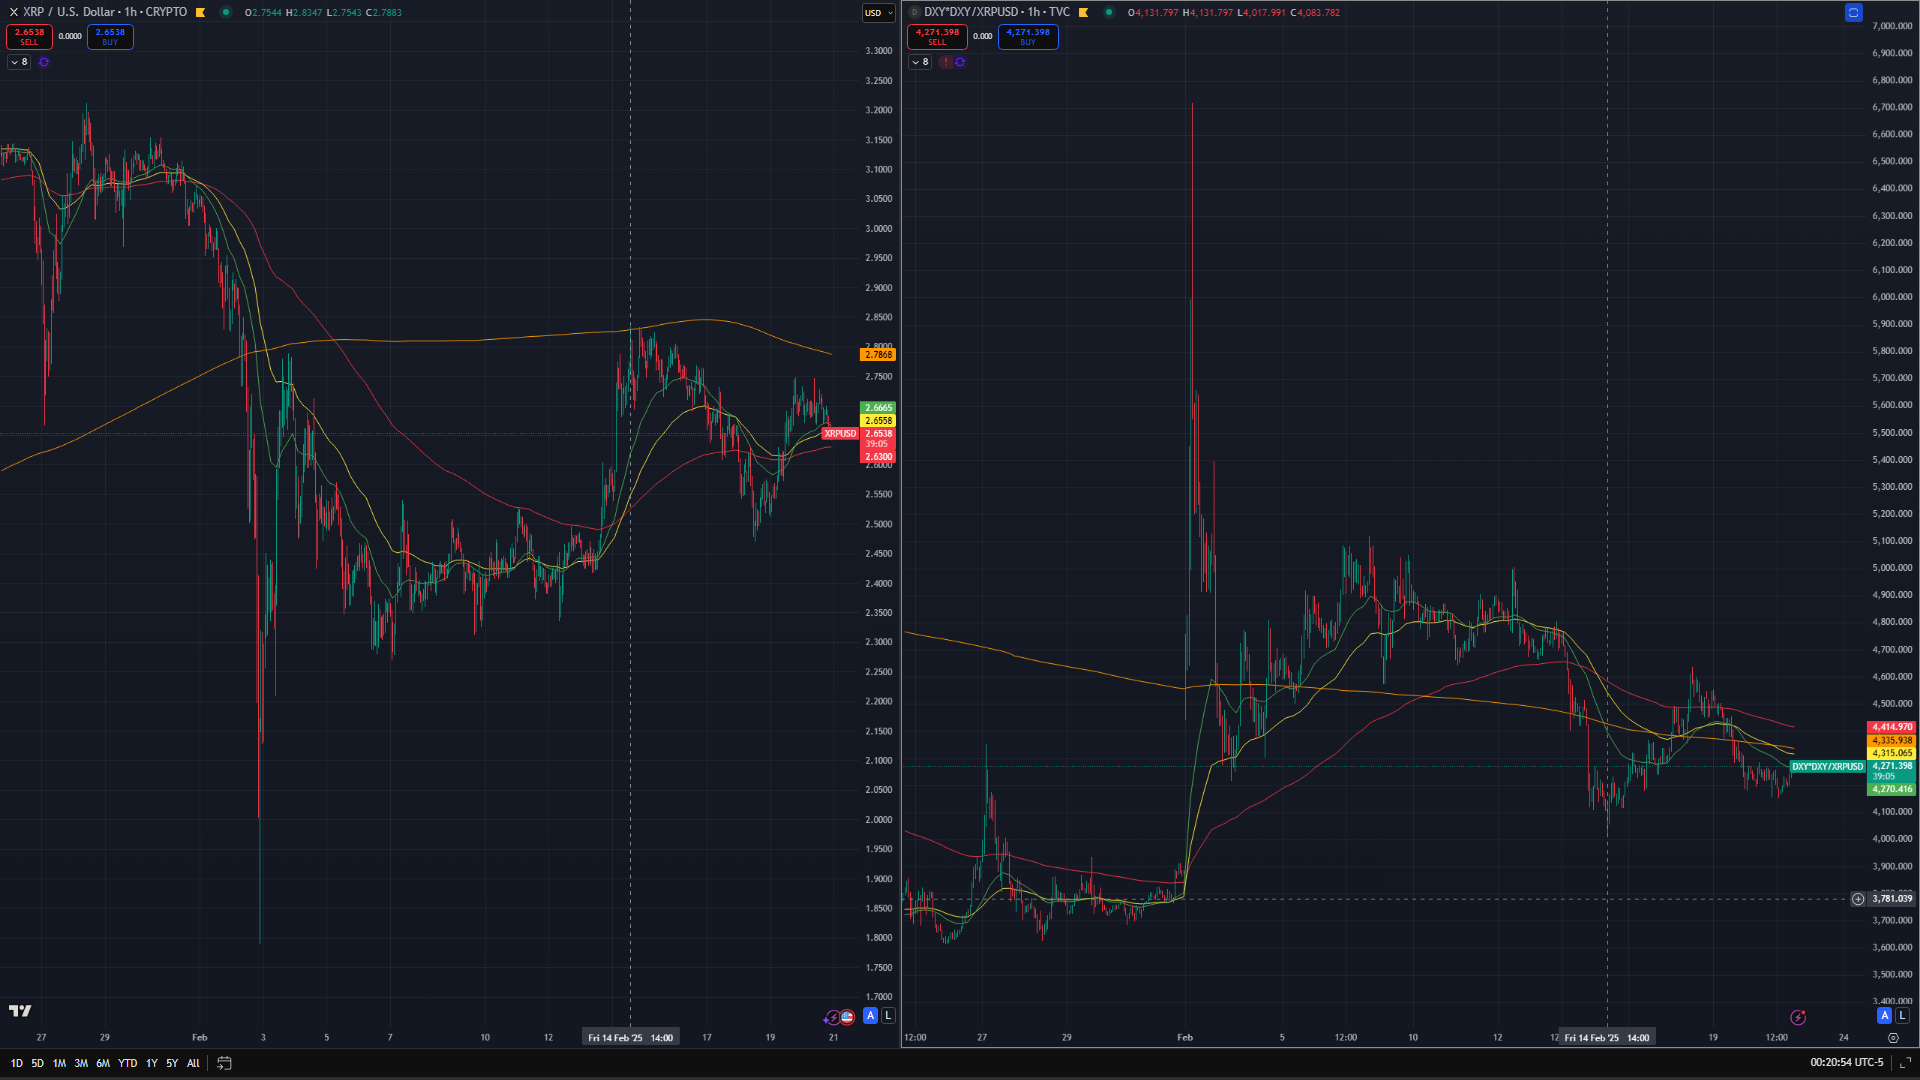
\includegraphics[width=0.3\textwidth]{one_hour_5.png}
\captionof


{Antifractal behavior observed in the (DXY)$^2$/XRPUSD metric at a 1-hour timeframe.}
\label{fig:onehour}
\end{minipage}
\end{center}

\subsection*{1-Day Timeframe Screenshots}
\begin{center}
\begin{minipage}{\textwidth}
\centering
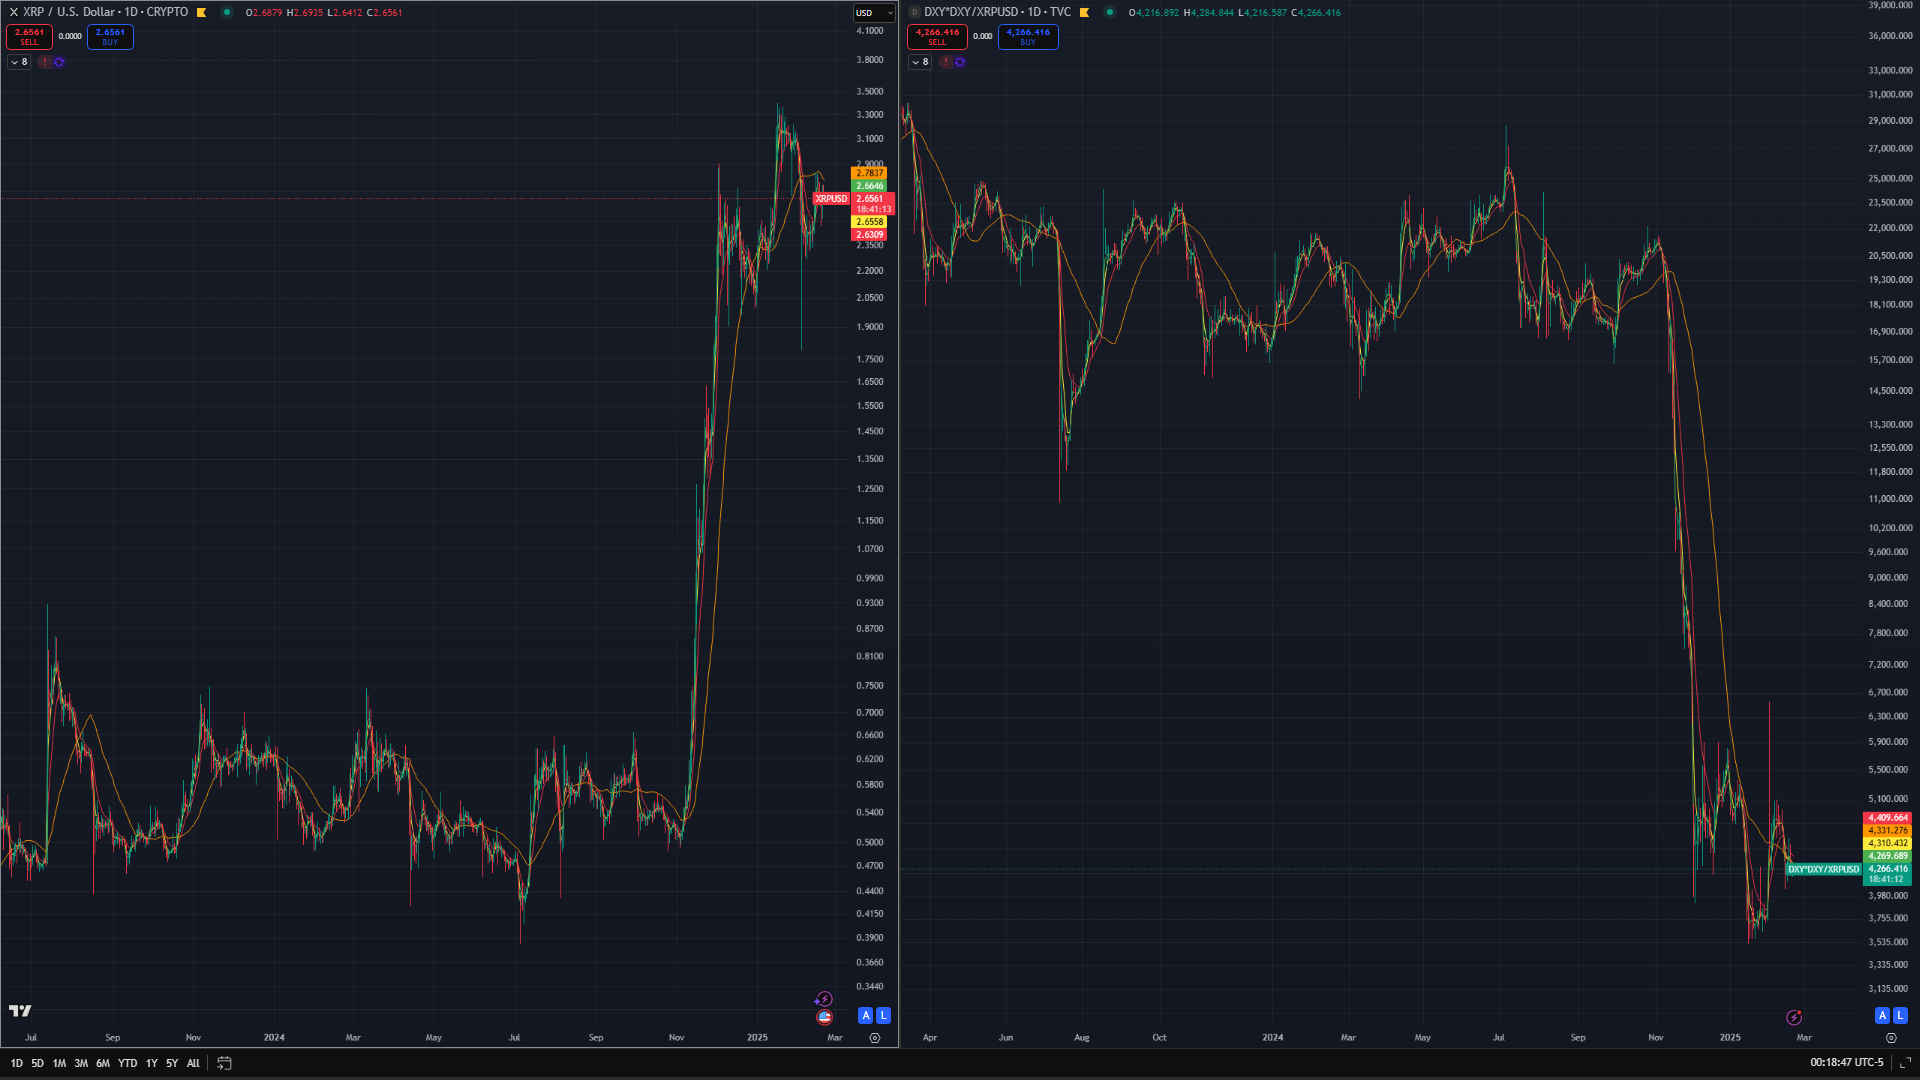
\includegraphics[width=0.3\textwidth]{one_day_1.png}
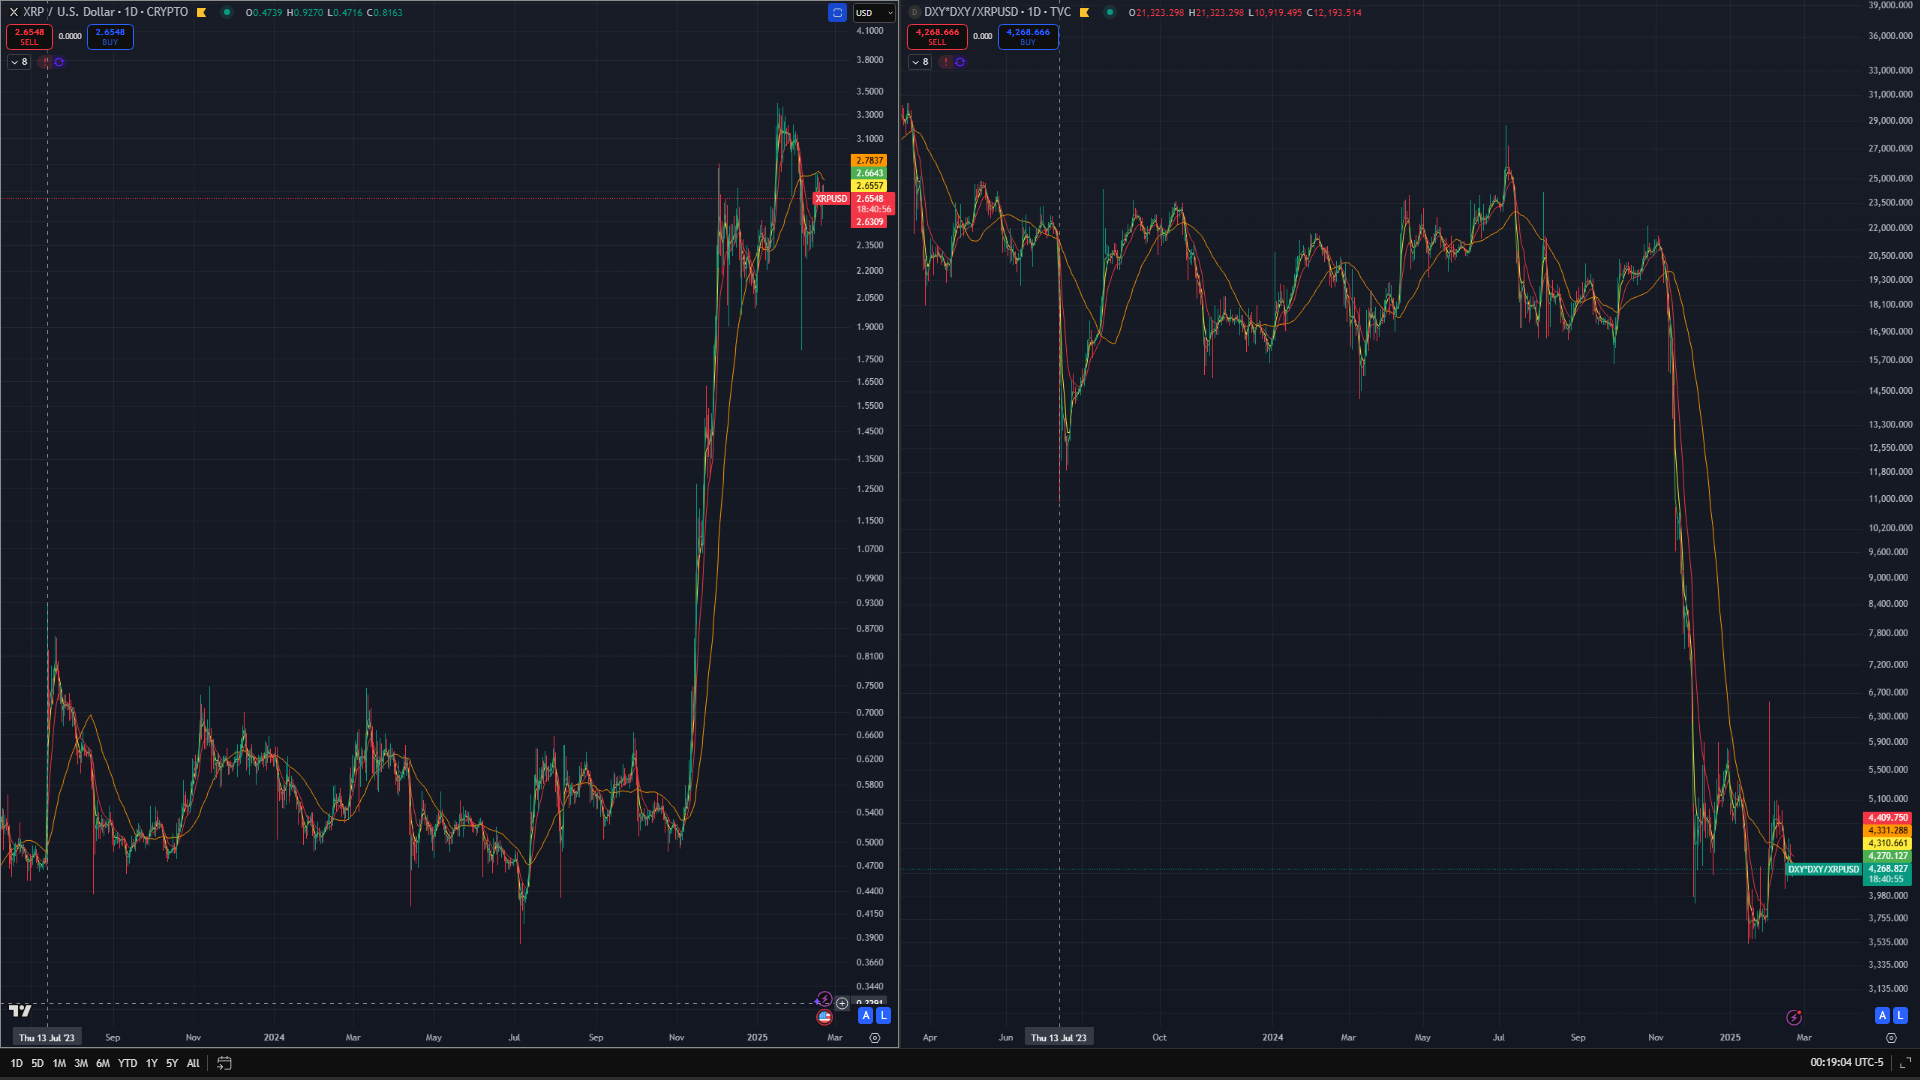
\includegraphics[width=0.3\textwidth]{one_day_2.png}
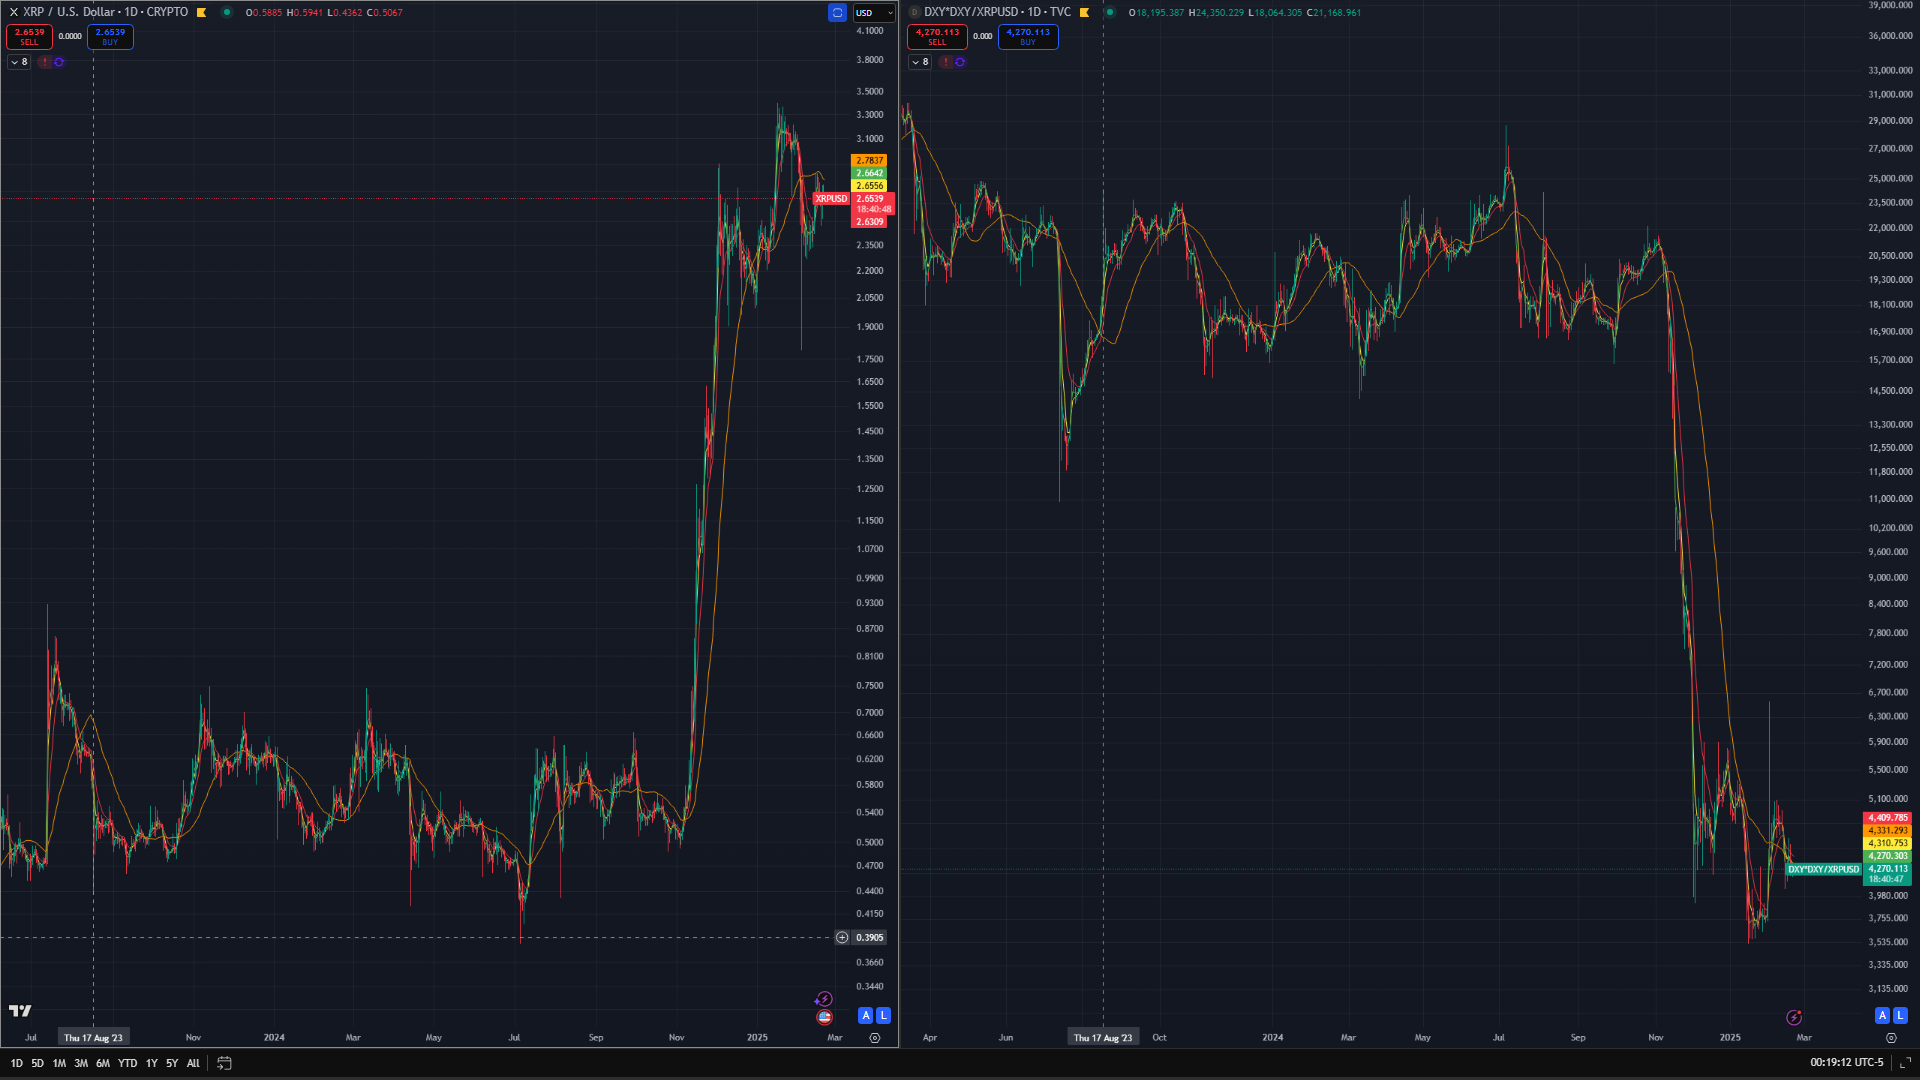
\includegraphics[width=0.3\textwidth]{one_day_3.png}\\[5mm]
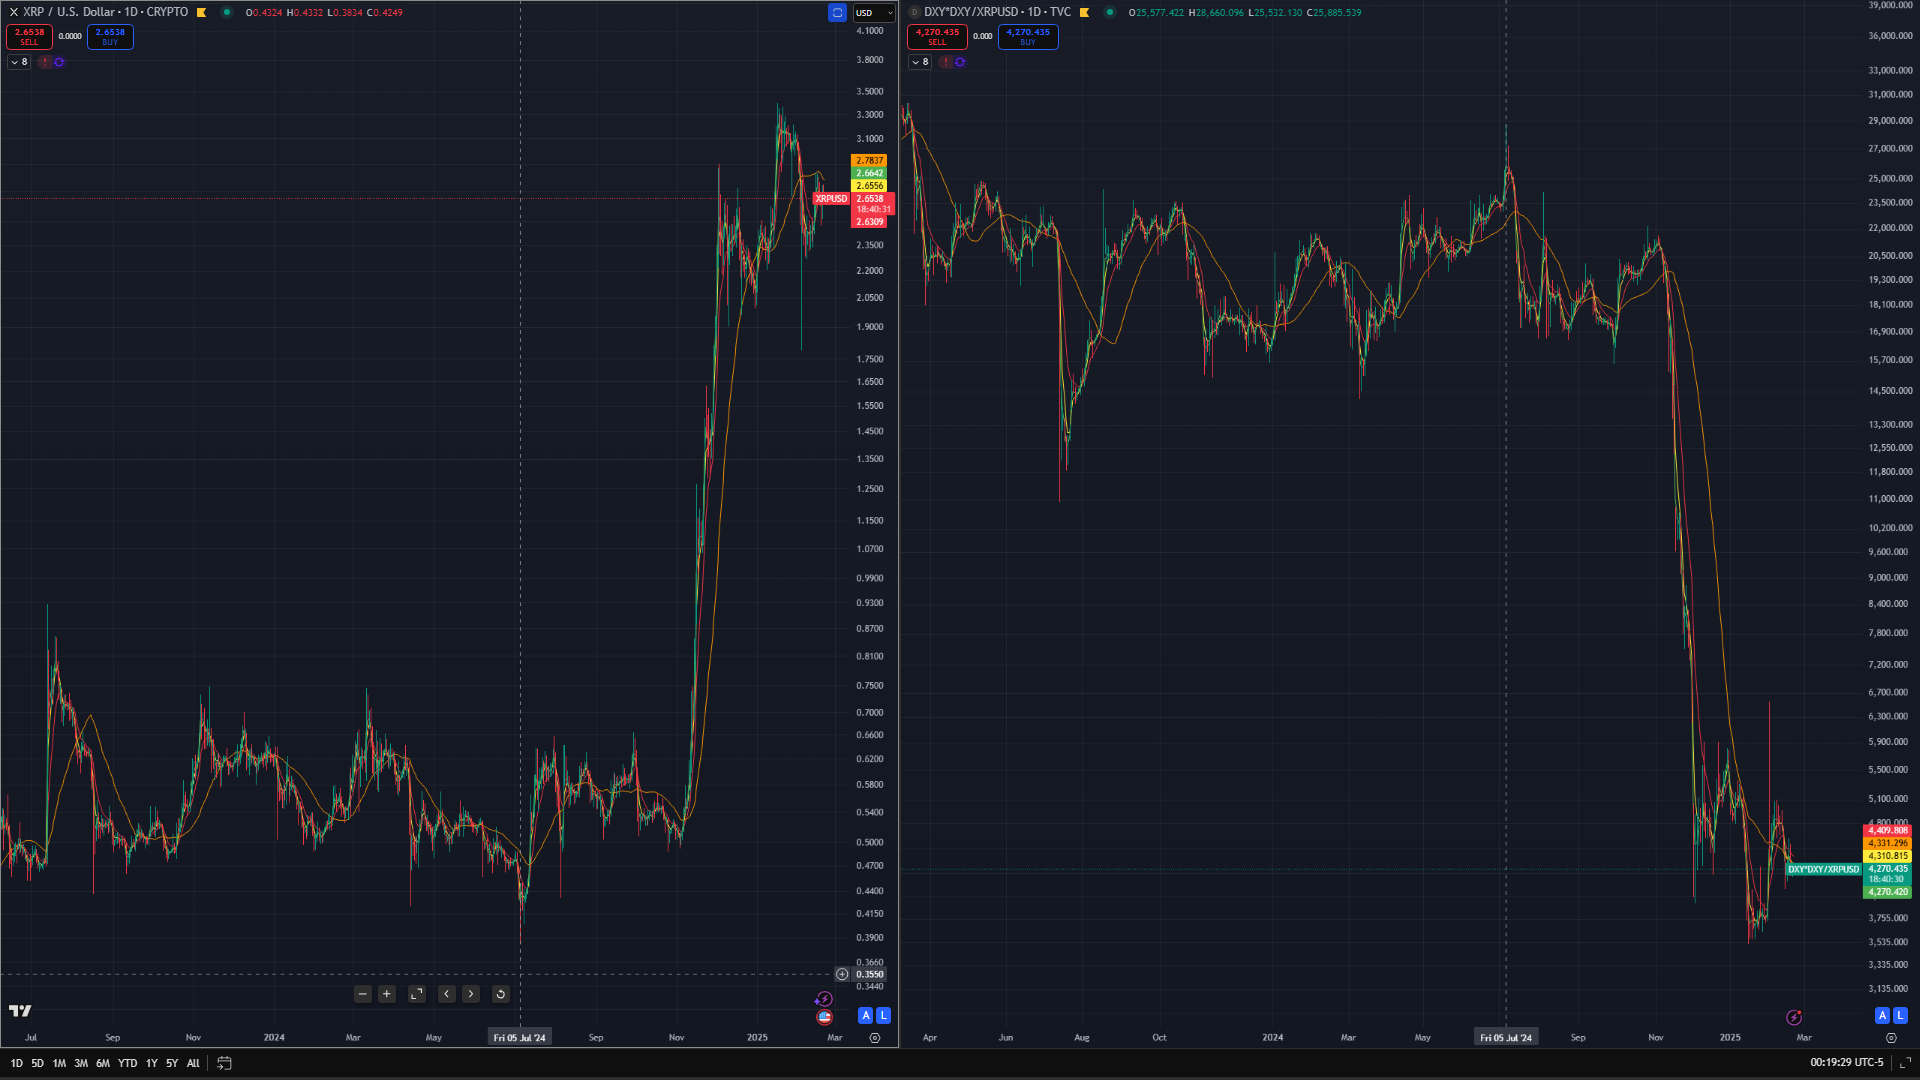
\includegraphics[width=0.3\textwidth]{one_day_4.png}
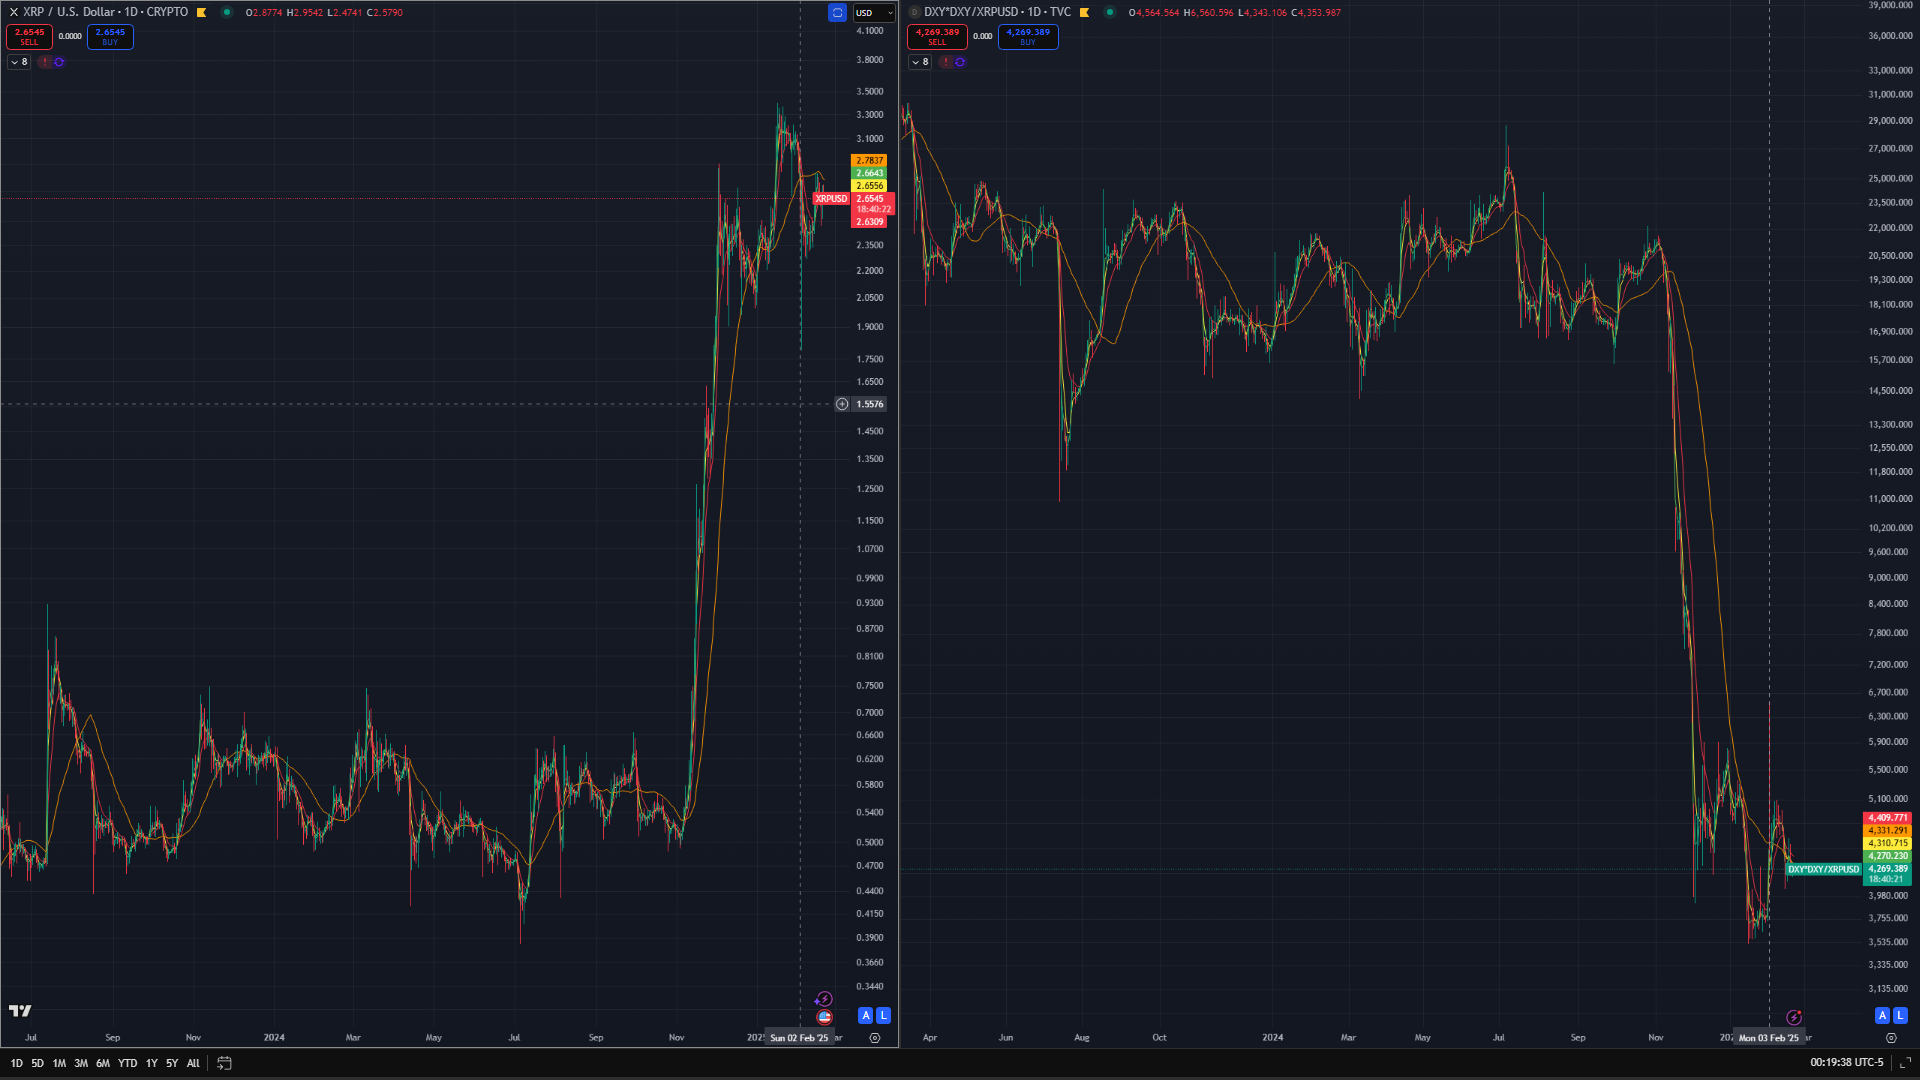
\includegraphics[width=0.3\textwidth]{one_day_5.png}
\captionof{             
\noindent\textbf{

\begin{center}
\textbf{Note on Logarithmic Scale:}
\end{center}
\vspace{2mm}
Using a logarithmic scale transforms multiplicative or exponential relationships into linear (additive) ones, which compresses the vertical axis and highlights relative changes. While on shorter timeframes (1 second, 1 minute, 1 hour) the antifractal relationship between XRPUSD and the custom spread (DXY$^2$/XRPUSD) is clearly visible in the raw data, on a daily timeframe large absolute differences can mask these subtle proportional trends. By applying a logarithmic scale, the data is normalized, revealing the underlying self-similar, antifractal patterns more clearly. This approach makes the dynamics easier to observe and understand for both laypersons and experts.



Antifractal behavior observed in the (DXY)$^2$/XRPUSD metric at a 1-day timeframe.}
\label{fig:onemin}
\end{minipage}
\end{center}





These groups collectively support the claim that both the macro (DXY) and micro (XRPUSD) markets operate under the same universal acceleration constant,k squared,which maps acceleration dynamics and energy flow across both macroscopic and microscopic systems back and forth so the operator can optimize their own subjective interpretation of throughput.

\subsection{Enhanced Information via Inverse Analysis}
By analyzing the acceleration of the inverse (logarithmic) function, the framework captures the complete recycling dynamics of a system, effectively doubling the available correlation information. This comprehensive insight is crucial for identifying conditions of maximum flux and optimizing energy throughput.

\section{Real-World Applications and Interdisciplinary Unification}
The universal \(K^2\) framework is applicable to every system since all fields involve transformations of energy, momentum, and time:
\begin{itemize}
    \item \textbf{Theoretical Physics \& Cosmology:} Unifies micro-level quantum fluctuations with macroscopic spacetime curvature, completing Einstein's unified field theory and refining black hole thermodynamics.
    \item \textbf{Finance \& Economics:} Replaces heuristic models with precise, probabilistic predictions by linking micro-scale liquidity fluctuations to macro-scale market trends, as demonstrated by antifractal behavior in the metric \((\text{DXY})^2/\text{XRPUSD}\).
    \item \textbf{Fluid Dynamics \& Engineering:} Provides robust models for turbulent flows, energy dissipation, and momentum transfer, optimizing the design of engines and industrial systems.
    \item \textbf{Biology \& Neuroscience:} Quantitatively connects micro-scale biochemical and neural processes with macro-scale organism behavior, offering insights into metabolism and the subjective acceleration of time.
    \item \textbf{Artificial Intelligence \& Data Science:} Enhances predictive algorithms by dynamically correlating micro-level data fluctuations with macro-scale outcomes.
    \item \textbf{Sustainable Energy \& Advanced Propulsion:} Suggests that nearly complete energy recycling is theoretically possible, opening pathways to revolutionary technologies such as cold fusion and optimized propulsion systems.
     \item \textbf{Quantum Computing} Probabalistic determination will leverage the intrinsic probability distributions of quantum states rather than pre-programmed heuristic search strategies. ie results will emerge from quantum state evoution rather than algorithmic aproximations. 
\end{itemize}
By performing acceleration analysis of the inverse (logarithmic) function, this framework captures the complete picture of system recycling dynamics—effectively doubling the available correlation information—and offers a comprehensive understanding of energy flow. Since any system can be regarded as a subset of a larger whole, the \(K^2\) transformation is universally applicable, laying the foundation for a new interdisciplinary field: Unified Systems Dynamics.

\section{Conclusion}
I have rigorously derived, from established first principles, a universal \(K^2\) transformation law that bridges micro- and macro-level dynamics. The derivation shows that
\[
p_{\text{micro}} = K \cdot p_{\text{macro}} \quad \text{and} \quad E_{\text{micro}} = K^2 \cdot E_{\text{macro}},
\]
confirming that energy and momentum transform predictably through the universal constant \(K^2\). Moreover, by performing acceleration analysis of the inverse (logarithmic) function, the framework captures the complete picture of system recycling dynamics, providing twice the available correlation information and a comprehensive understanding of energy flow. This unified model not only completes the integration of quantum mechanics with general relativity---as envisioned by Einstein and refined by Hawking---but also offers transformative applications across finance, fluid dynamics, biology, artificial intelligence, sustainable energy, and more.

\bigskip
My unified field acceleration model describes how energy flow and acceleration dynamics bridge macroscopic and microscopic systems.As it correctly maps the transformation of energy and momentum across different time scales then an operator (user of the model) can optimize their subjective interpretation of throughput-ie tuning the system based on their chosen parameters or desired outcomes.

\bigskip
I propose that this universal transformation model represents a paradigm shift in our understanding of energy, momentum, and time. By replacing heuristic approximations with precise, probabilistic predictions, the \(K^2\) framework lays the foundation for a new interdisciplinary field, Unified Systems Dynamics, dedicated to optimizing system performance in every aspect of science and everyday life.

\bigskip
\section*{References}
\begin{thebibliography}{99}
\bibitem{Kreyszig} Kreyszig, E. (2011). \textit{Advanced Engineering Mathematics} (10th ed.). Wiley.
\bibitem{Arfken} Arfken, G. B., Weber, H. J., \& Harris, F. E. (2012). \textit{Mathematical Methods for Physicists} (7th ed.). Elsevier.
\bibitem{Misner} Misner, C. W., Thorne, K. S., \& Wheeler, J. A. (1973). \textit{Gravitation}. W. H. Freeman.
\bibitem{Hawking74} Hawking, S. W. (1974). Black hole explosions? \textit{Nature}, 248(5443), 30--31.
\bibitem{Hawking75} Hawking, S. W. (1975). Particle creation by black holes. \textit{Communications in Mathematical Physics}, 43(3), 199--220.
\bibitem{Griffiths} Griffiths, D. J. (2018). \textit{Introduction to Quantum Mechanics} (3rd ed.). Cambridge University Press.
\bibitem{Strogatz} Strogatz, S. H. (2018). \textit{Nonlinear Dynamics and Chaos: With Applications to Physics, Biology, Chemistry, and Engineering} (2nd ed.). Westview Press.
\bibitem{Mandelbrot} Mandelbrot, B. B. (1983). \textit{The Fractal Geometry of Nature}. W. H. Freeman.
\bibitem{Bertalanffy} von Bertalanffy, L. (1968). \textit{General System Theory: Foundations, Development, Applications}. George Braziller.
\bibitem{Hirsch} Hirsch, M. W., Smale, S., \& Devaney, R. L. (2012). \textit{Differential Equations, Dynamical Systems, and an Introduction to Chaos} (3rd ed.). Academic Press.
\bibitem{Econophysics} Sinha, S., Chatterjee, A., Chakraborti, A., \& Chakrabarti, B. K. (2010). \textit{Econophysics: An Introduction}. Cambridge University Press.
\end{thebibliography}

\end{document}

